%Autor: Piotr Woźniak
\documentclass[12pt, twoside, openany]{mwrep}
\usepackage{polski}
\usepackage[T1]{fontenc}
\usepackage[utf8]{inputenc}
\usepackage{graphicx}
\usepackage[a4paper,top=25mm,bottom=25mm,left=30mm,right=20mm,bindingoffset=0mm]{geometry}
\usepackage{blindtext}
\usepackage{helvet}
\usepackage{fancyhdr}
\usepackage{fontspec}
%\usepackage{enumerate}
\usepackage{amssymb}
\usepackage{amsmath}
\usepackage{mathrsfs}
\usepackage[usenames, dvipsnames]{color}
\usepackage{gensymb}
\usepackage{float}
\usepackage{cite}
\usepackage[chapter]{algorithm}
\usepackage{mleftright}
\usepackage[noend]{algpseudocode}
\usepackage{lipsum}
%\usepackage{enumitem}
\usepackage{fontspec}

\graphicspath{ {./images/} }

\newcommand{\lnn}[1]{%
  \ln\left(#1\right)%
}

\newcommand{\lnb}[1]{%
  \ln\mleft(#1\mright)%
}

\floatname{algorithm}{Kod}

\renewcommand{\algorithmicrequire}{\textbf{Na wejściu:}}
\renewcommand{\algorithmicensure}{\textbf{Na wyjściu:}}
\renewcommand{\algorithmicprocedure}{\textbf{funkcja}}

\renewcommand{\listalgorithmname}{Listingi kodu}

\renewcommand{\labelitemi}{$\bullet$}

\DeclareMathOperator{\sign}{sign}

%%%%%czcionki
\setromanfont[
BoldFont=timesbd.ttf,
ItalicFont=timesi.ttf,
BoldItalicFont=timesbi.ttf,
]{times.ttf}

\setsansfont[
BoldFont=arialbd.ttf,
ItalicFont=ariali.ttf,
BoldItalicFont=arialbi.ttf
]{arial.ttf}
%%%%%

\linespread{1.15}
\setlength{\parindent}{0.5cm}

\pagestyle{fancy}
\fancyhead{}
\renewcommand{\chaptermark}[1]{\markboth{\thechapter.\ #1}{}}
\fancyhead[RO]{\nouppercase{\leftmark}}
\fancyhead[LE]{\nouppercase{\rightmark}}
\renewcommand{\headrulewidth}{0.4pt}
\fancyfoot{}
\fancyfoot[LE,RO]{\thepage}

\fancypagestyle{opening}{%
  \fancyhf{}\fancyfoot[LE,RO]{\thepage}%
  \renewcommand{\headrulewidth}{0pt}}
  
\fancypagestyle{closing}{%
  \fancyhf{}\fancyhead[RO]{\nouppercase{\leftmark}}\fancyhead[LE]{\nouppercase{\rightmark}}\fancyfoot[LE,RO]{\thepage}%
  \renewcommand{\headrulewidth}{0.4pt}}
  

\newtheorem{theorem}{Twierdzenie}[section]

\begin{document}

%--------------------------------------------------------------
%Strona tytułowa
\begin{titlepage}
    \begin{center}
        %{\fontfamily{phv}\selectfont
        {\sffamily
            \begin{center}
                
\includegraphics[width=\textwidth]{titlepage/szablonEITI.png}\\   
            \end{center}
            \hfill \break
            \hfill \break
            Instytut Mikroelektroniki i Optoelektroniki\\
            \hfill \break
            \hfill \break
            \begin{center}
                
\includegraphics[width=\textwidth]{titlepage/szablonINZ.png}\\
            \end{center}
            na~kierunku Elektronika\\
            w~specjalności Elektronika i Inżynieria Komputerowa\\
            \hfill \break
            \hfill \break
            \large
            Konstrukcja dedykowanej stacji usługowej Internetu Rzeczy z zastosowaniem komputera jednopłytkowego.\\
            \hfill \break
            \hfill \break
            \LARGE
            Marcin Michał Piotrowski\\
            \normalsize
            Numer albumu 300346\\
            \hfill \break
            \hfill \break
            promotor\\
            dr~hab. inż. Michał Borecki, prof. PW\\
            \vfill
            WARSZAWA 2022
        }
    \end{center}
    \newpage
    \thispagestyle{empty}
    \hfill
    
    \newpage

\end{titlepage}
%-----------------------------------------------------------------------------------------

\thispagestyle{empty}
\newpage
\hyphenation{Syl-ves-tra}
\hyphenation{Syl-ves-ter-a}

\newpage
\setcounter{page}{1}

%------------------------------------------------------------------------------
%Streszczenie PL
\thispagestyle{empty}
\centerline{\bf Streszczenie}
\centerline\textit\noindent{\bf Tytuł:}
Konstrukcja dedykowanej stacji usługowej Internetu Rzeczy z zastosowaniem komputera jednopłytkowego.
   \hfill \break
\par
Niniejsza praca ma na celu konstrukcje urządzenia służącego do bezprzewodowej integracji węzłów sieci Internetu Rzeczy, oraz przeprowadzenie jego weryfikacji eksperymentalnej w zmieniających się warunkach.  
\par
W ramach projektu skonfigurowano komputer jednopłytkowy, aby pełnił funkcje serwera, stworzono dedykowane oprogramowanie oraz dokonano projektu węzła wraz z jego konstrukcją. Następnie porównano wpływy zakłóceń innymi sygnałami oraz fizycznych przeszkód obecnych w bloku mieszkalnym i jednorodzinnym domu w celu ustalenia warunków niezawodnej komunikacji bezprzewodowej.
   \hfill \break
   \hfill \break
\textbf{Słowa kluczowe:} Internet Rzeczy, komputer jednopłytkowy, łączność bezprzewodowa
\clearpage
%------------------------------------------------------------------------------
%------------------------------------------------------------------------------
%Streszczenie ENG
\thispagestyle{empty}
\centerline{\bf Abstract}
\centerline\textit\noindent{\bf Title:}
Construction of a dedicated Internet of Things service station using a single board computer.
   \hfill \break
	\par 
The aim of this work is to construct a device for wireless integration of the Internet of Things nodes, and conduct its experimental verification under changing conditions.
\par
As part of the project, a single-board computer was configured to act as a server, dedicated software was created and the node was designed together with its construction. They then compared the interference effects of other signals and the physical obstacles present in the apartment block and the single-family house to establish conditions for reliable wireless communication.
   \hfill \break
   \hfill \break
\textbf{Keywords:} Internet of Things, single board computer, wireless connectivity
%------------------------------------------------------------------------------
\newpage
\thispagestyle{empty}
\begin{figure}[H]
\vspace{-55pt}%
\noindent\makebox[\textwidth]{%
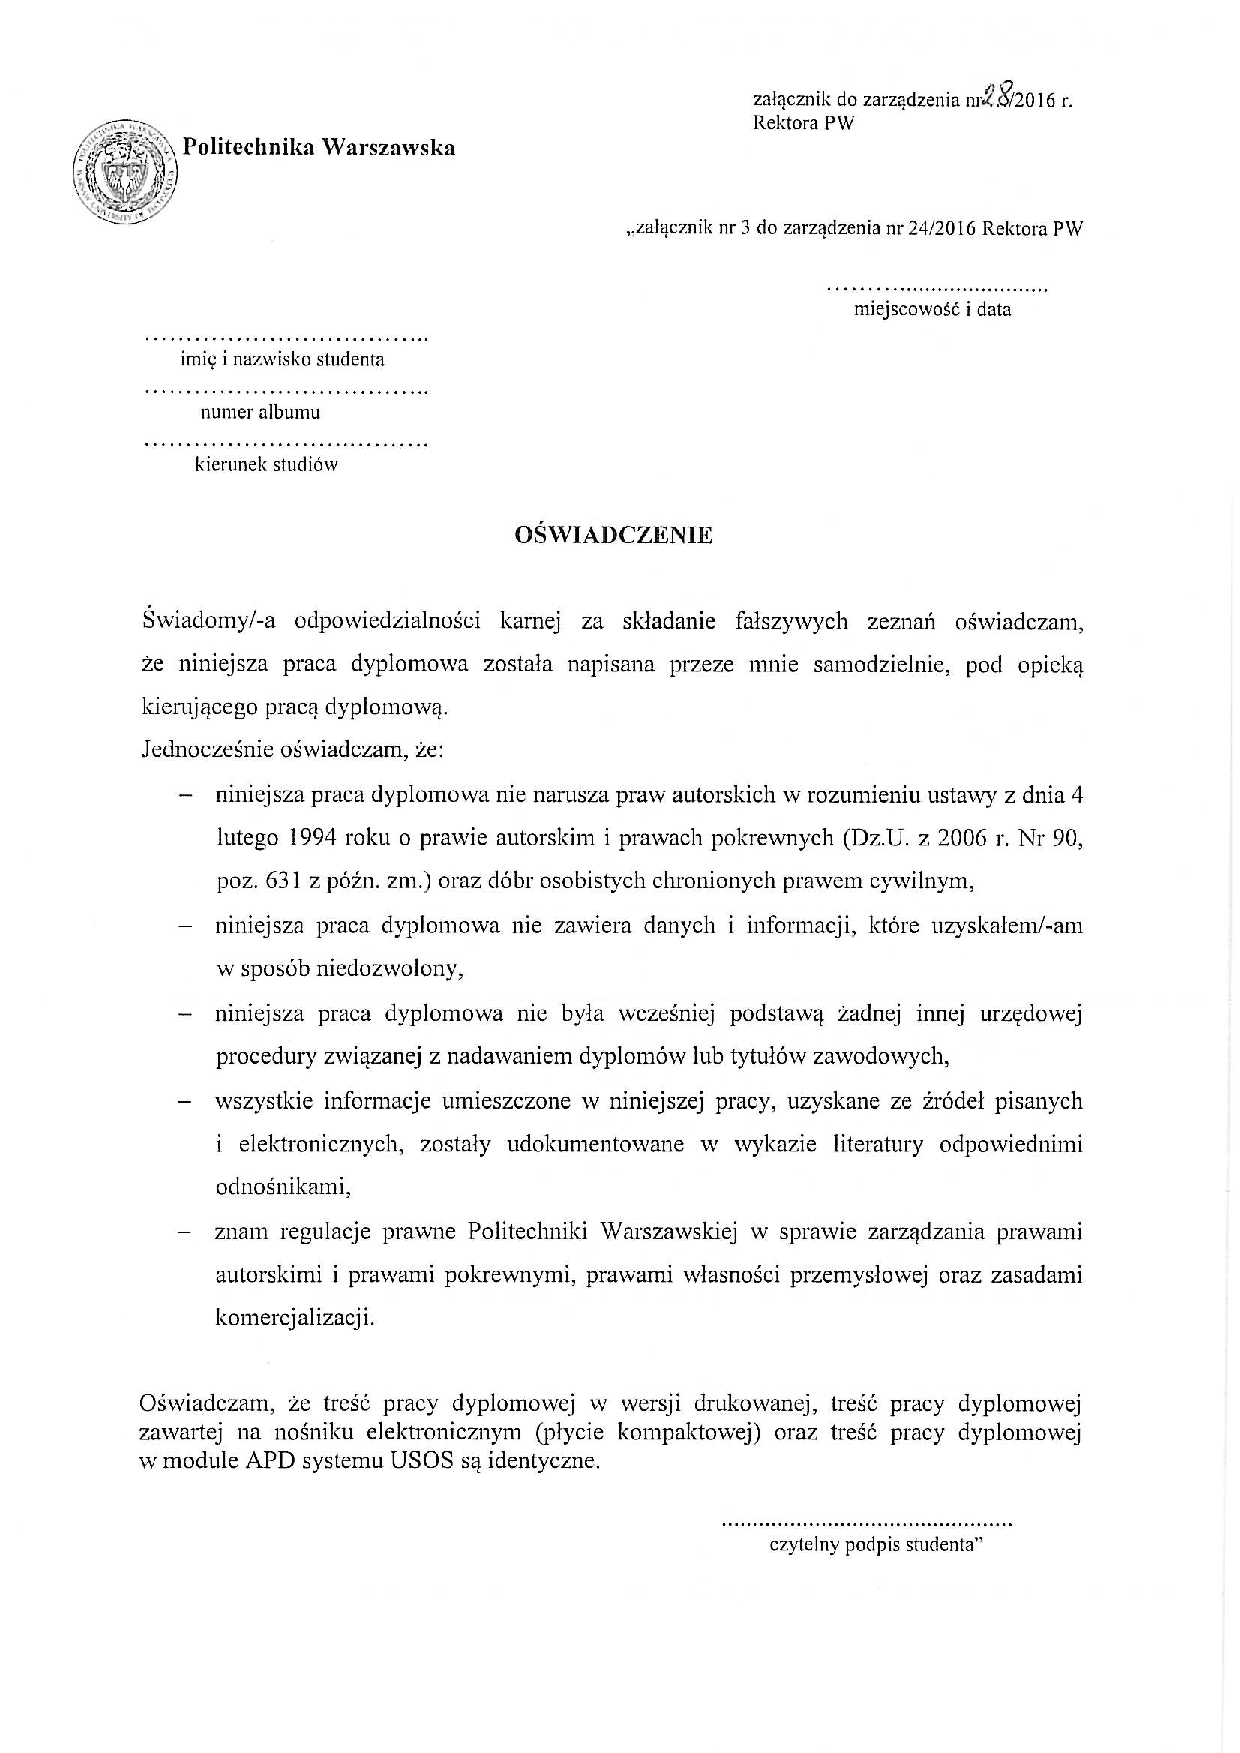
\includegraphics[width=1.3\textwidth]{./pdfs/2strona.pdf}}
\end{figure}
\newpage

%Spis treści
\tableofcontents
\clearpage

%------------------------------------------------------------------------------
%----POCZĄTEK----
\chapter{Wstęp}
\par
Internet Rzeczy jest to koncepcja wedle której rozmaite przedmioty mają pozyskiwać i przetwarzać dane oraz komunikować się ze sobą w celu współpracy. Wprowadzenie tego typu rozwiązań ma na celu usprawnienie wszystkich dziedzin naszego życia poprzez optymalizacje kosztów i zużycia energii. W literaturze i biznesie idea ta najczęściej określana jest anglojęzycznym skrótowcem IoT (Internet of Things).
\par
Analizując dane rynkowe można zaobserwować gwałtowny wzrost popularności Internetu Rzeczy. W 2017 wartość światowego rynku IoT przekroczyła 100 miliardów dolarów, z czego prognozowane jest, że w 2024 będzie wynosić ponad bilion dolarów [9]. Jest to tym bardziej imponujące, jeśli weźmiemy pod uwagę jak młoda jest ta koncepcja. Według raportu Cisco Systems [1] Internet Rzeczy powstał na przełomie 2008 i 2009 roku, kiedy liczba połączonych ze sobą „rzeczy” przewyższyła liczbę ludzi na ziemi.
Obecną sytuację zawdzięczamy przede wszystkim dynamicznemu rozwojowi takich dziedzin nauki jak elektronika, telekomunikacja i informatyka. To właśnie dzięki nim możliwe jest skonstruowanie urządzeń dostarczających kluczowe dane, komunikacja przy użyciu zaawansowanych protokołów i przetwarzanie ogromnej ilości informacji w chmurze. W efekcie na rynku pojawiło się mnóstwo urządzeń określanych mianem inteligentnych (ang. smart) które potrafią porozumiewać się ze sobą i światem zewnętrznym. Prognozowane jest, że do 2025 roku na świecie będzie około 25 miliardów urządzeń określanych mianem IoT. Tak prężny rozwój może oznaczać, że Internet Rzeczy zdominuje praktycznie każdą dziedzinę naszego życia tak jak zrobił to dotychczas Internet ludzi.
\par
Obecna sytuacja stanowi ogromne wyzwanie dla konstruktorów, aby dostarczyć użytkownikom gotowe rozwiązania, które umożliwią im czerpanie korzyści jakie niesie za sobą IoT. Jednym z problemów, który wymaga rozwiązania jest integracja ogromnej liczby urządzeń i tym samym umożliwienie użytkownikom tworzenie własnych inteligentnych systemów. Rozwiązaniem tego problemu jest stacja usługowa Internetu Rzeczy, której konstrukcja jest tematem niniejszej pracy. Stacja taka stanowi interfejs dla człowieka tak aby mógł on łatwo stworzyć inteligentną sieć i pozyskiwać z niej potrzebne informacje.
\par
\section{Cele pracy}
Nniejsza praca ma na celu:
\begin{itemize}
    \item zaprojektowanie stacji usługowej Internetu Rzeczy z zastosowaniem komputera jednopłytkowego,
    \item konstrukcja wersji demonstracyjnej,
    \item przeprowadzenie testów w celu sprawdzenia czy zostały spełnione założenia projektu.
\end{itemize}   

%----2------
\chapter{Internet rzeczy od strony użytkownika}

%----2.1------
\section{Zastosowania Internetu Rzeczy}

Główne założenie Internetu Rzeczy w postaci sieci komunikujących się ze sobą urządzeń sprawia, że może znaleźć on zastosowanie praktycznie wszędzie. W kolejnych latach rozwoju tej koncepcji będą odkrywane kolejne jej zastosowania niemniej już można wyróżnić kilka najpopularniejszych.
\par
Pierwszym najbardziej popularnym zastosowaniem IoT jest użycie go w gospodarstwie domowym.  Większość naszego życia spędzimy właśnie w domu, dlatego nawet niewielkie usprawnienia w zakresie oszczędzania energii bądź automatyzacji mogą przynieść znaczne korzyści. W obecnych czasach w prawie każdym domu obecna jest bez przewodowa sieć Wi-Fi która stanowi świetny kanał komunikacji dla wszelkiego rodzaju urządzeń. Inteligentny dom charakteryzuje się pełną automatyką w zakresie sterowania oświetleniem, roletami bądź termostatem. Wszystko odbywa się w oparciu o zdalnie sterowane przekaźniki, dane z czujników bądź zewnętrznych źródeł. Możliwe również jest bieżące monitorowanie z dowolnego miejsca na ziemi informacji takich jak które okna i drzwi są otwarte, zużycie mediów czy obraz z monitoringu [2]. Wszystkie urządzenia takiego systemu są integrowane i wchodzą w interakcje z użytkownikiem poprzez dedykowaną stacje usługową Internetu Rzeczy.
\par
Kolejnym obszarem, w którym Internet Rzeczy może przynieść wiele korzyści jest rolnictwo. Dla rolnika kluczowe jest zapewnienie roślinom dobrych warunków do wzrostu poprzez odpowiednie nawożenie i nawodnienie. Internet Rzeczy oferuje rozwiązanie tego problemu w postaci siatki czujników umieszczonych głęboko w glebie monitorujących jej parametry [3]. Na podstawie informacji z takiego systemu oraz zewnętrznych danych meteorologicznych możliwe jest optymalne zaplanowanie nawadniania oraz ograniczenie ilości środków ochrony roślin do niezbędnego minimum.
\par
Monitorowanie parametrów gleby, powietrza i wody może nieść również za sobą szersze korzyści. Innym zastosowaniem Internetu Rzeczy jest przewidywanie nadchodzących klęsk żywiołowych takich jak powodzie, trzęsienia ziemi czy huragany [3]. Architektura służących w tym celu systemów ma postać sieci, w której węzłami są komunikujące się ze sobą czujniki. W ten sposób możliwe jest pokrycie dużych obszarów tak aby wykrywać zbliżające się niebezpieczeństwa z odpowiednim wyprzedzeniem i zapewnić okolicznej ludności czas na ewakuacje.
\par
Innym obszarem naszego życia, w którym Internet Rzeczy może okazać się pomocny jest medycyna. Wiele ludzi dopiero dostrzega, że ma problemy ze zdrowiem, gdy ich stan znacząco się pogorszy, dlatego tak ważnym zadaniem jest ciągłe monitorowanie parametrów życiowych takich jak ciśnienie krwi, tętno czy poziom glukozy. Według koncepcji IoT może się to odbywać za pomocą urządzeń noszonych bezpośrednio na ciele pacjenta. Urządzenia takie łączą się z Internetem poprzez standard LTE lub w przypadku chęci uzyskania niskiego poboru prądu można wykorzystać identyfikacje radiową (RFID). Rozwiązania takie są w stanie częściowo wyręczyć lekarza i zmniejszyć ilość okresowych wizyt oraz dostarczyć informacje o nagłym pogorszeniu stanu zdrowia pacjenta [4].
\par
Ostatnim obszarem, w którym w którym Internet Rzeczy powoli zaczyna zmieniać rzeczywistość jest przemysł. Dzieje się to za sprawą trwającej czwartej rewolucji przemysłowej (ang. Industry 4.0) która stanowi koncepcje według której nastąpi automatyzacja większości procesów przemysłowych między innymi za sprawą IoT. Urzeczywistnieniem tej idei jest inteligentna fabryka, w której maszyny tworzące linię produkcyjną są sterowane przez oprogramowanie, które podejmuje decyzje na podstawie danych z czujników bez ludzkiej interwencji. Przykładem tego, że ta rewolucja już się zaczęła jest chociażby złożony proces palenia kawy, który udało się zautomatyzować dzięki rozwiązaniom, które oferuje Internet Rzeczy [5].

%----2.2------
\section{Przegląd technologii}

Szerokie zastosowanie Internetu Rzeczy stawia różnorodne wymagania sprzętowe w kwestii interakcji z maszynami. Z tego powodu w tej dziedzinie stosuje się wszelkiego rodzaju systemy wbudowane ze względu na ich uniwersalność i różnorodność.  Urządzenia stosowane w IoT można podzielić na trzy grupy, gdzie w skład pierwszej grupy wchodzą systemy o najmniejszej mocy obliczeniowej i ilości pamięci operacyjnej, z kolei urządzenia w trzeciej grupie dorównują mocą obliczeniową komputerom osobistym [6]. 
\par
Pierwsza grupa składa się z urządzeń, które charakteryzują się zazwyczaj 8 bądź 16 bitową architekturą procesora i pamięcią RAM liczoną w dziesiątkach kilobajtów. Oznacza to, że niemożliwe jest na nich uruchomienie systemu operacyjnego takiego jak Windows bądź Linux, więc do programowania takich urządzeń wykorzystuje się niskopoziomowe języki jak na przykład C. Tak mocno ograniczone zasoby sprzętowe sprawiają, że urządzenia z tej grupy posiadają niską cenę oraz zużycie energii i wymiary. Stosuje się je głównie w czujnikach, gdzie jedynym zadaniem jest dokonanie pomiaru i przesłanie jego wyniku dalej poprzez określony protokół. 
\par
Urządzenia w drugiej grupie to również systemy mikroprocesorowe z tą różnicą, że posiadają większą moc obliczeniową względem pierwszej grupy. W przypadku tych urządzeń parametry takie jak taktowanie procesora i ilość pamięci RAM przyjmują wartości rzędu setek mega herców i kilobajtów. Jest to wystarczająca ilość zasobów, aby możliwe było przetwarzanie zebranych danych w celu na przykład rozpoznawania obrazu lub dźwięku. Ceny urządzeń z tej grupy są równie niskie jak w przypadku pierwszej grupy, lecz wyższe taktowanie procesora powoduje większe zużycie energii co może być problemem, jeśli zależy nam na zasilaniu bateryjnym.
\par
Trzecia grupa składa się z jednopłytkowych komputerów, które pomimo wymiarów karty płatniczej posiadają podobną ilość zasobów do komputerów osobistych.  Oznacza to, że można na nich uruchomić system operacyjny taki jaki Windows bądź Linux przez co do ich programowania da się wykorzystać wysokopoziomowe języki jak na przykład Python. Tak duża moc obliczeniowa umożliwia wykonywanie skomplikowanych zadań takich jak algorytmy szyfrowania i kryptografii bądź pełnienie funkcji serwera. Urządzenia z tej grupy często są stosowane jako stacje usługowe Internetu Rzeczy, gdyż dobrze sobie radzą z obsługą dużej ilości zadań na raz takich jak komunikacja z innymi urządzeniami, przetwarzanie danych i obsługa żądań. Zużycie energii w tym przypadku jest największe, na przykład najpopularniejszy jednopłytkowy komputer dostępny na rynku, czyli Raspberry Pi potrzebuje średnio 4 watów mocy, dlatego musi być zasilany poprzez sieciowy adapter.

%----2.3------
\section{Koncepcje komunikacji bezprzewodowej}

Nieodłącznym elementem Internetu Rzeczy jest łączność bezprzewodowa, dlatego warto przybliżyć związane z nią koncepcje. Wszystkie z nich cechują się innym zastosowaniem z uwagi na osiągalne parametry takie jak zasięg, zużycie energii i koszt przez co znajdują zastosowanie w różnych dziedzinach życia.

%----2.3.1.------
\subsection{Rodzaje sieci}

Sieci bezprzewodowe wykorzystywane między innymi w Internecie Rzeczy można klasyfikować ze względu na zasięg i rodzaj urządzeń, które ze sobą łączą. Poniżej zestawiono kilka wariantów począwszy od tych o najmniejszym zasięgu i skończywszy na największym.
\begin{itemize}
    \item Sieć typu BAN (ang. Body Area Network) jest to sieć tworzona z urządzeń noszonych przez człowieka [12]. Mogą to być wszczepiane w ciało implanty, urządzenia przytwierdzane do powierzchni ciała lub noszone w kieszeni [13]. Interakcja takiej sieci ze światem zewnętrznym odbywa za pośrednictwem urządzenia, które ma bezpośredni dostęp do Internetu, czyli tzw. bramki, dzisiaj najczęściej jest to smartfon.
    \item Sieć prywatna PAN (ang. Personal Area Network) łączy urządzenia w obrębie miejsca pracy pojedynczej osoby [14]. Przykładem takiej sieci może być komputer wraz z bezprzewodowymi urządzeniami peryferyjnymi takimi jak mysz i klawiatura. Jeśli komputer ma dostęp do Internetu pełni wtedy również pełni funkcje bramki.
    \item Lokalna sieć LAN (ang. Local Area Network) łączy ze sobą co najmniej dwa komputery na ograniczonym obszarze takim jak gospodarstwo domowe, uczelnia bądź biurowiec [15]. Tym co wyróżnia ją spośród wcześniej wymienionych sieci jest to, że wykorzystuje ona pakiet protokołów internetowych TCP/IP. Dzięki temu lokalna sieć daje namiastkę „zwykłego” Internetu, gdyż korzysta się z niej przy użyciu takich samych narzędzi. Istnieją również odmiany sieci LAN jak na przykład MAN (ang. Metropolitan Area Network) czyli sieci o zasięgu całych miast, lecz zasada ich działania pozostaje taka sama.
    \item Globalna Sieć WAN (ang. Wide Area Network) jest to sieć, która obejmuje swoim zasięgiem całe państwa czy kontynenty. Największym i najbardziej znanym przykładem sieci WAN o zasięgu prawie całego globu jest Internet [16]. Jak łatwo się domyślić wykorzystuje on pakiet protokołów internetowych TCP/IP przez co można również podłączać do niego mniejsze, lokalne sieci LAN o podobnej architekturze.
\end{itemize}   

\begin{figure}[H]
\centering
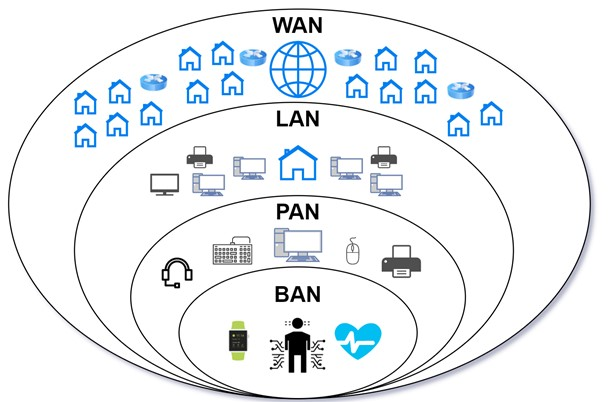
\includegraphics[scale=0.9]{rodzaje_sieci}
\caption{Diagram różnych rodzajów sieci}
\end{figure}

%----2.3.2.------
\subsection{Topologie sieci}

Innym kryterium, na które można podzielić sieci Internetu Rzeczy i nie tylko jest sposób w jaki węzły komunikują się ze sobą. Poszczególne konfiguracje są nazywane topologiami wraz ze kształtem, który najlepiej oddaje ich wygląd. Poniżej opisano najczęściej spotykane rodzaje.
\begin{itemize}
    \item Gwiazda – w tej topologii wszystkie węzły są podłączone do jednego punktu, gdzie punkt centralny pełni również funkcje bramki do świata zewnętrznego. Jej główną zaletą jest prostota, oraz fakt, że awaria peryferyjnego węzła nie ma wpływu na działanie całej sieci. Z drugiej strony prostota może okazać się wadą, ponieważ w przypadku awarii centralnego punktu cała sieć przestaje działać.
    \item Siatka – w tym przypadku każdy z węzłów ma połączenie z paroma sąsiednimi węzłami. Zaletą tej topologii jest to, że punkt centralny pełniący funkcje bramki nie musi mieć bezpośredniego połączenia z każdym węzłem, więc można uzyskać pokrycie dużego obszaru niższym kosztem niż w przypadku gwiazdy. Inną korzyścią jest większa niezawodność komunikacji, gdyż zawsze istnieje droga alternatywna w przypadku awarii jednego węzłów. Potencjalną wadą może być skomplikowany proces trasowania pakietów, który wymaga większej mocy obliczeniowej co przekłada się na większy pobór prądu.
    \item Mieszana – jest to połączenie dwóch lub więcej topologii w jedną sieć. Stosuję się ją w celu wykorzystania zalet bądź ominięcia ograniczeń danej topologii w newralgicznych punktach.
\end{itemize}

\begin{figure}[H]
\centering
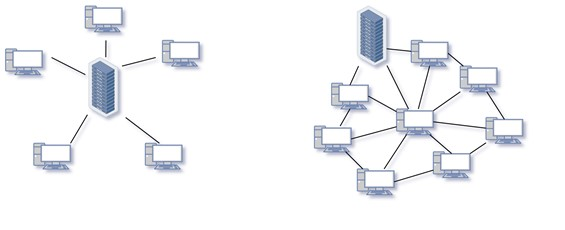
\includegraphics[scale=1.2]{gwiazda_siatka}
\caption{Przykłady topologii sieci, po lewej stronie topologia gwiazdy, po prawej stronie topologia siatki}
\end{figure}
\hfill \break
\begin{figure}[H]
\centering
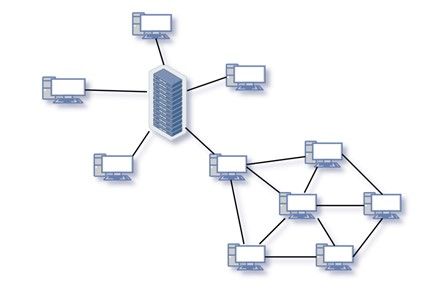
\includegraphics[scale=1.2]{mieszana}
\caption{Topologia mieszana}
\end{figure}

%----2.4------
\section{Standardy komunikacji bezprzewodowej}

W obecnych czasach stosowane są rozmaite standardy komunikacji bezprzewodowej z czego wszystkie oparte są o fale elektromagnetyczne w zakresie częstotliwości od 3 kHz do 3000GHz [17] zwane również falami radiowymi. Z tego powodu trzeba być świadomym wykorzystywanego pasma częstotliwości, ponieważ tylko wąski zakres spośród wszystkich użytecznych pasm został wydzielony przez ministra administracji i cyfryzacji do bezpłatnego i swobodnego korzystania [11]. Takim zakresem jest pasmo ISM (ang. Industrial, Scientific and Medical) służące do zastosowań przemysłowych, naukowych i medycznych w skład, którego wchodzą częstotliwości 2.4 GHz i 5 GHz. Większość z opisywanych w tej pracy technologii będzie korzystać z pasma 2.4 GHz, ponieważ zapewnia ono lepszą propagację sygnału w porównaniu do 5 GHz i zadowalającą szybkość transmisji.

%----2.4.1.------
\subsection{Wi-Fi}

Wi-Fi jest technologią opartą na standardzie IEEE 802.11 i od początku było projektowane jako bezprzewodowy zamiennik dla standardu IEEE 802.3, czyli Ethernet. Najbardziej powszechnym jej zastosowaniem jest tworzenie lokalnych sieci LAN, gdzie router Wi-Fi pełni funkcje punktu centralnego w topologii gwiazdy. 
\par
Wi-Fi od samego początku, czyli od 1997 roku w ramach standardu IEEE 802.11 korzysta z pasma 2,4 GHz, które jest podzielone na 13 kanałów. Takie rozwiązanie ma wadę w postaci problemów z siłą oraz stabilnością sygnału, ponieważ częstotliwość 2,4 GHz jest wykorzystywana również przez kamery, smartfony, głośniki Bluetooth czy kuchenki mikrofalowe. W konsekwencji pasmo to jest przeciążone co szczególnie daje się we znaki mieszkańcom bloków mieszkalnych w postaci kiepskiego zasięgu. Rozwiązaniem tego problemu ma być wprowadzone wraz z kolejnymi wersjami standardu 802.11 w 2003 roku pasmo 5 GHz. Jest to częstotliwość nie wykorzystywana przez domowe sprzęty i do tego została podzielona na większą liczbę, szerszych kanałów wynoszącą 19, co w teorii powinno zapewnić lepszą stabilność sygnału i szybkość transmisji [18]. 
\par
Pomimo możliwości interferencji z innymi urządzeniami to właśnie częstotliwość 2,4 GHz zapewnia większy zasięg. Jest to spowodowane tym, że sama fala jest dłuższa niż w przypadku 5 GHz przez co jest mniej podatna na zakłócenia powodowane przez przeszkody terenowe takie jak drzwi, ściany czy meble. Efektywnie przekłada się to na od kilkunastu do kilkudziesięciu metrów zasięgu. Popularne modele routerów Wi-Fi dostępnych na rynku pracujące na częstotliwości 2,4 GHz są w stanie bez problemu zapewnić dostęp do Internetu w całym, średniej wielkości domu podczas gdy w przypadku 5 GHz zasięg często kończy się kilka metrów dalej od nadajnika. Najlepiej to ilustrują poniższe rysunki 2.4 i 2.5 na których przedstawiono moce poszczególnych sygnałów Wi-Fi o różnych częstotliwościach zmierzone w jednym z bloków mieszkalnych w Warszawie. Wyraźnie na nich widać, że pasmo 5 GHz, poza tym, że ma więcej kanałów, nie jest tak przeciążone jak pasmo 2,4 GHz.
\hfill \break
\begin{figure}[H]
\centering
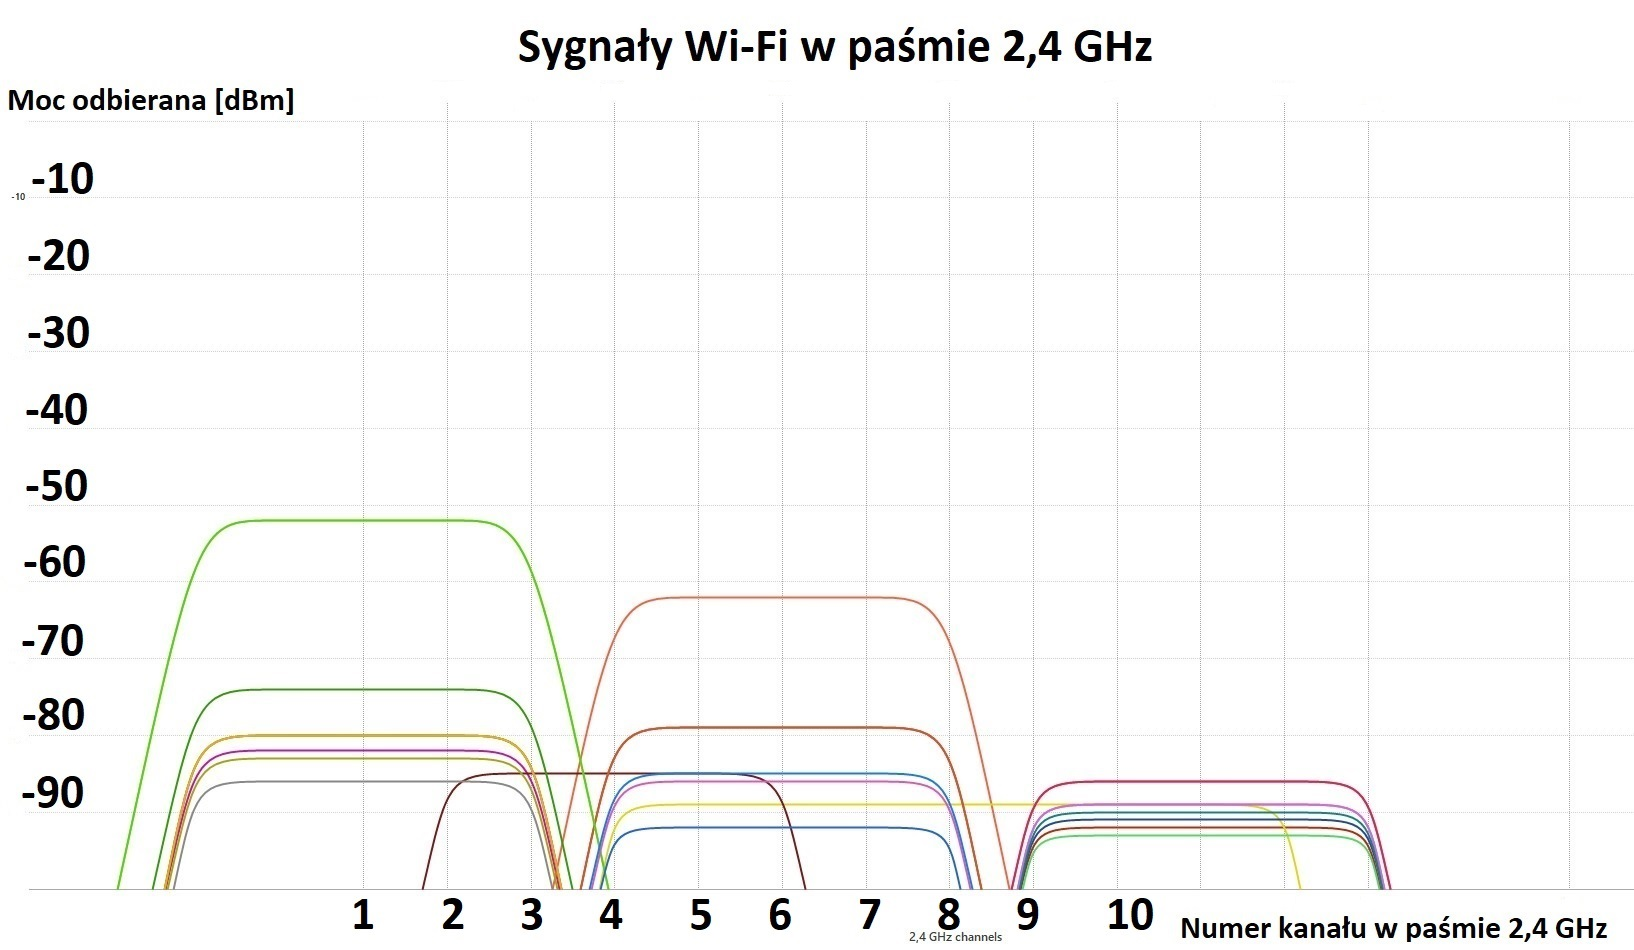
\includegraphics[scale=0.35]{2,4GHz}
\caption{Moce poszczególnych sygnałów Wi-Fi w paśmie 2,4 GHz}
\end{figure}
\begin{figure}[H]
\centering
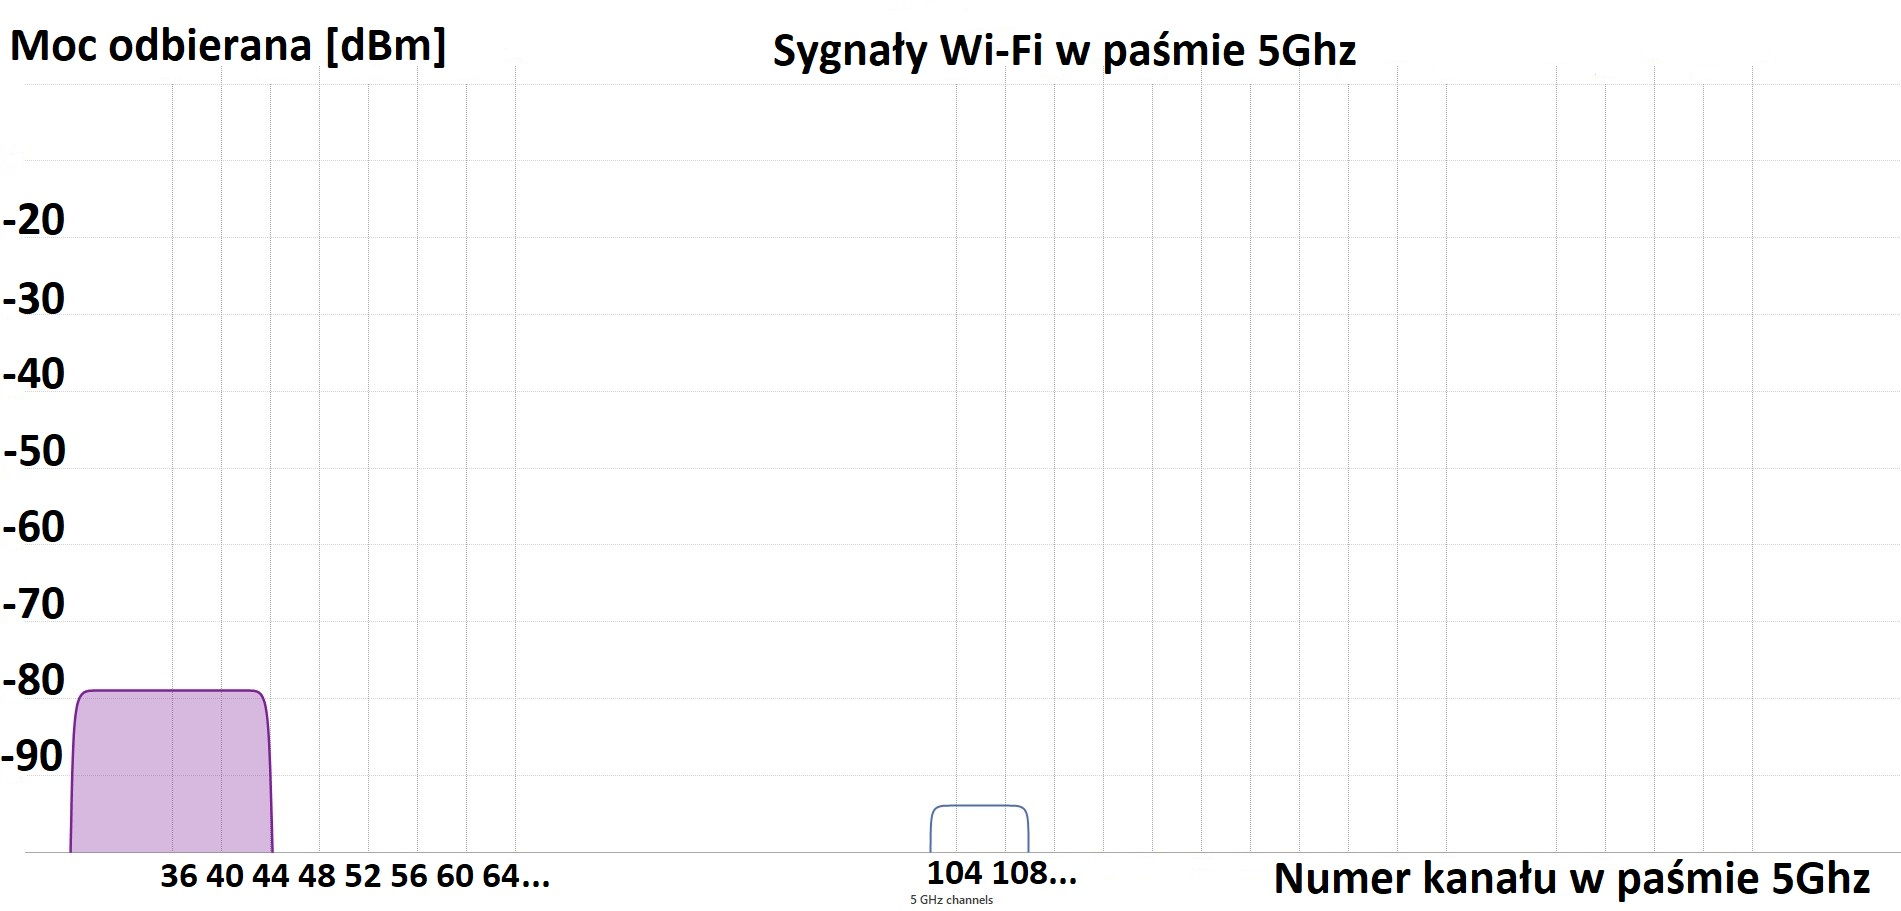
\includegraphics[scale=0.35]{5GHz}
\caption{Moce poszczególnych sygnałów Wi-Fi w paśmie 5 GHz}
\end{figure}

\par
Z racji, iż w obecnych czasach sieć Wi-Fi jest dosłownie wszędzie oczywiste jest, że znajduje zastosowanie również w Internecie Rzeczy. Na rynku już istnieje wiele rozwiązań w postaci gotowych modułów wraz z zaimplementowanym stosem protokołów TCP/IP i wbudowaną anteną co pozwala bardzo łatwo stworzyć urządzenie łączące się ze światem zewnętrznym poprzez Wi-Fi. Niestety poważną wadą takich systemów jest wysoki pobór prądu, który sprawia, że nie nadają się do zasilania przy użyciu baterii. Z tego powodu w sieciach Internetu Rzeczy czujniki zasilane bateryjnie komunikują się wykorzystując bardziej energooszczędne standardy.

%----2.4.2.------
\subsection{Bluetooth}

Bluetooth określany też skrótowcem BT wykorzystuje fale radiowe o częstotliwości 2,4 GHz do przesyłania danych między urządzeniami na niewielkie odległości. Od Wi-Fi różni się pod tym względem, że komunikacja odbywa się bezpośrednio pomiędzy dwoma urządzeniami. Oznacza to, że dwa urządzenia wyposażone w Bluetooth mogą wymieniać informacje między sobą, podczas gdy w przypadku Wi-Fi zawsze będzie wymagany router, który pośredniczy w tym procesie. Zasięg Bluetooth wynosi teoretycznie około 10 metrów w najpopularniejszej klasie mocy 2.5mW [21], a szybkość transmisji to 2.1 MB/s w trybie EDR (ang. Enchanced Data Rate) o zwiększonej szybkości transmisji.  Jest to znacznie mniej niż w przypadku Wi-Fi, gdzie przy odpowiednim umieszczeniu routera skuteczny zasięg może być kilkukrotnie większy, a szybkość transmisji dla nowych standardów zaczyna się od 600 MB/s [20]. Ma to bezpośredni związek z zużyciem energii, gdzie to właśnie Bluetooth jest postrzegany jako standard bardziej energooszczędny. Przykładowo Wi-Fi pobiera około 500 µW energii elektrycznej przy wysłaniu 10 wiadomości dziennie podczas gdy Bluetooth w wersji Low Energy blisko 10 razy mniej [19].
\par
W zastosowaniach IoT Bluetooth sprawdza się wszędzie tam, gdzie wymagane jest zasilanie bateryjne. Niewątpliwą zaletą jest to, że dzisiaj każdy smartfon czy komputer posiadają wbudowany interfejs BT, więc mogą pełnić one funkcję wcześniej omawianej bramki Wi-Fi. Dodatkowym atutem może być również wprowadzona w 2017 możliwość konstruowania sieci o topologii siatki nazywana Bluetooth Mesh. Pozwala ona na ominięcie ograniczeń BT w postaci niskiego zasięgu przy założeniu, że dysponujemy gęsto upakowaną siecią węzłów. 

%----2.5------
\section{Prywatność i bezpieczeństwo}

Prywatność i bezpieczeństwo użytkowników Internetu Rzeczy stanowi istotny problem, który dalej nie został do końca rozwiązany. Faktem jest, że rozmaite urządzenia często w niejasny sposób gromadzą informacje w celu zapewnienia spersonalizowanych doświadczeń. Budzi to uzasadniony niepokój dotyczący tego, gdzie gromadzone są nasze dane, kto ma do nich dostęp i czy są bezpieczne. Inną istotną kwestią jest często brak wystarczających zabezpieczeń w produktach dostępnych na rynku, co czyni je podatnymi na ataki hackerskie. Nawet na pozór nie przydatne dane takie jak temperatura i wilgotność powietrza w pomieszczeniu, mogą stanowić wrażliwą informację o tym czy dom jest pusty [7].
\par
W 2019 roku przeprowadzono badanie na grupie 25 osób, aby ustalić czego oczekują w temacie bezpieczeństwa od inteligentnego domu [7]. Najczęściej pojawiającymi się odpowiedziami była przejrzystość gromadzonych danych i kontrola nad nimi. Użytkownicy w momencie, kiedy nie są informowani jakie dane są gromadzone zaczynają podejrzewać, że w każdej chwili są inwigilowani. Z tego też powodu uczestnicy domagali się opcji tymczasowego wyłączenia zbierania danych w widoczny, sprzętowy sposób jak na przykład klucz w postaci wtyku USB. Inną sugestią wysuniętą w stronę konstruktorów było stwierdzenie, że nie wszystkie urządzenia muszą mieć dostęp do Internetu, a dane można przechowywać lokalnie zamiast w chmurze. Jednocześnie uczestnicy twierdzili, że są producenci, których darzą wystarczającym zaufaniem, aby bez obaw powierzyć im swoje dane. Powyższe badanie pokazuje, że poza samą ochroną danych poprzez stosowanie odpowiednich algorytmów i architektury równie ważna jest świadomość użytkownika i zaangażowanie go w ten proces.
\par
Poza zapewnieniem subiektywnego odczucia bezpieczeństwa użytkownikowi oczywiście trzeba o nie zadbać w fizyczny sposób. Głównym czynnikiem, który utrudnia te zadanie są ograniczone zasoby sprzętowe urządzeń tworzących inteligentne systemy. Urządzenia z pierwszej i drugiej grupy nie są przystosowane do szyfrowania danych w konwencjonalny sposób przy pomocy klucza publicznego. Wymusza to na konstruktorach stosowanie architektury z środkową warstwą aplikacji (ang. middleware), w której jest ona odpowiedzialna za przydzielanie każdemu urządzeniu unikalnej tożsamości w celu późniejszej identyfikacji [8]. W takiej konfiguracji urządzenia tworzące dany system nie komunikują się bezpośrednio ze światem zewnętrznym, lecz robią to poprzez bramkę, czyli na przykład smartfon bądź komputer jednopłytkowy który podłączony jest do Internetu. Bramka w czasie rzeczywistym wysyła zebrane dane oraz żądania o identyfikacje za pośrednictwem protokołu HTTP do Internetu. Żądania oraz nadchodzące dane są odbierane przez środkową warstwę aplikacji, która komunikuje się z bazą danych oraz przedstawia zebrane informacje użytkownikowi w przystępnej formie. 
\begin{figure}[H]
\centering
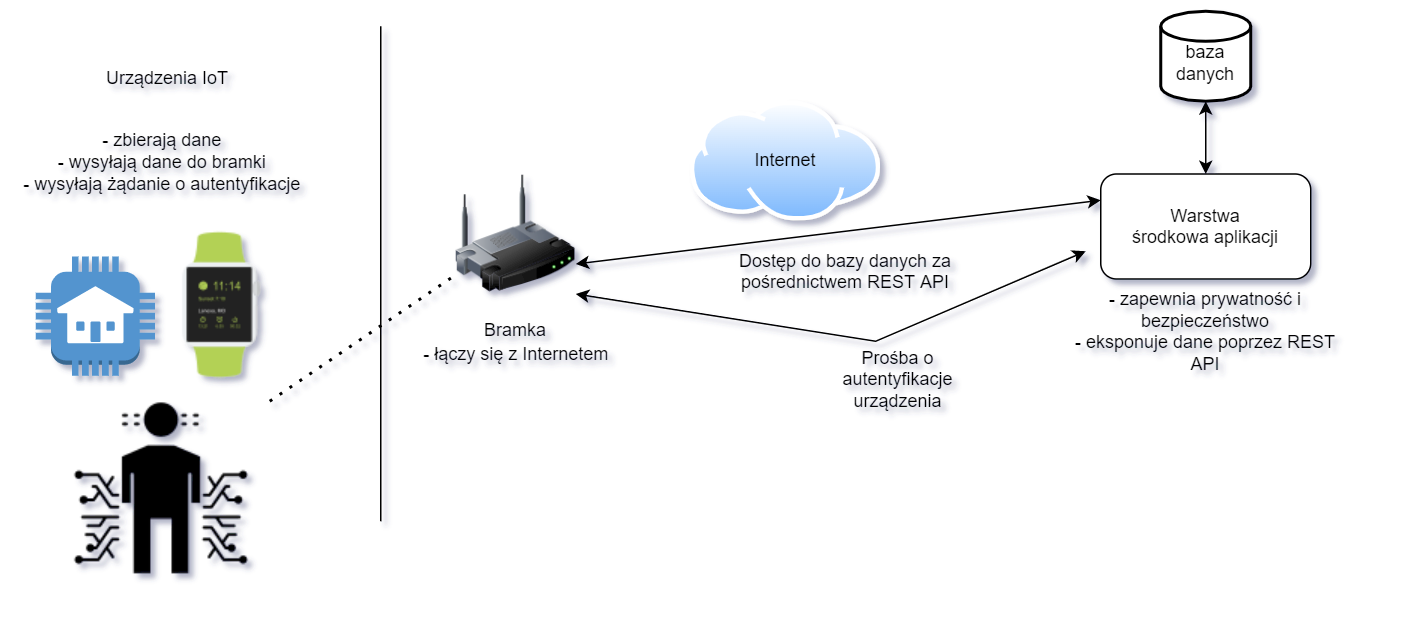
\includegraphics[scale=0.5]{bezpieczenstwo}
\caption{Schemat blokowy opisywanej architektury}
\end{figure}

%----3------
\chapter{Cel projektu}

Celem projektu jest konstrukcja stacji usługowej Internetu Rzeczy z zastosowaniem komputera jednopłytkowego. Do najważniejszych funkcjonalności stacji należą:
\begin{itemize}
\item	Dostarczenie użytkownikowi interfejsu do tworzenia sieci urządzeń.
\item	Gromadzenie danych pochodzących z węzłów sieci.
\item	Umożliwienie użytkownikowi komunikacji z węzłami z dowolnego miejsca.
\item	Zapewnienie prywatności i bezpieczeństwa użytkownikowi.
\end{itemize}
Aby osiągnąć powyższy cel przyjęto następujące założenia:
\begin{itemize}
\item	Oprogramowanie uruchomione na komputerze jednopłytkowym pełni funkcje serwera, który obsługuje żądania dodania nowego urządzenia do sieci, komunikacji z węzłami i podglądu gromadzonych danych.
\item	Stacja posiada graficzny interfejs użytkownika będący aplikacją Internetową dostępną za pośrednictwem protokołu http.
\item	Węzeł to urządzenie, które może pełnić dowolną funkcję w sieci.
\item	Węzły komunikują się ze stacją w sposób bezprzewodowy.
\item Każdy węzeł jest wykonany według określonego standardu i posiada unikatowy identyfikator.
\item	Dane są gromadzone lokalnie w pamięci komputera jednopłytkowego i tylko użytkownik ma do nich dostęp. 
\end{itemize}
Wizualizacją powyższych celów i założeń jest następujący schemat blokowy:
\begin{figure}[H]
\centering
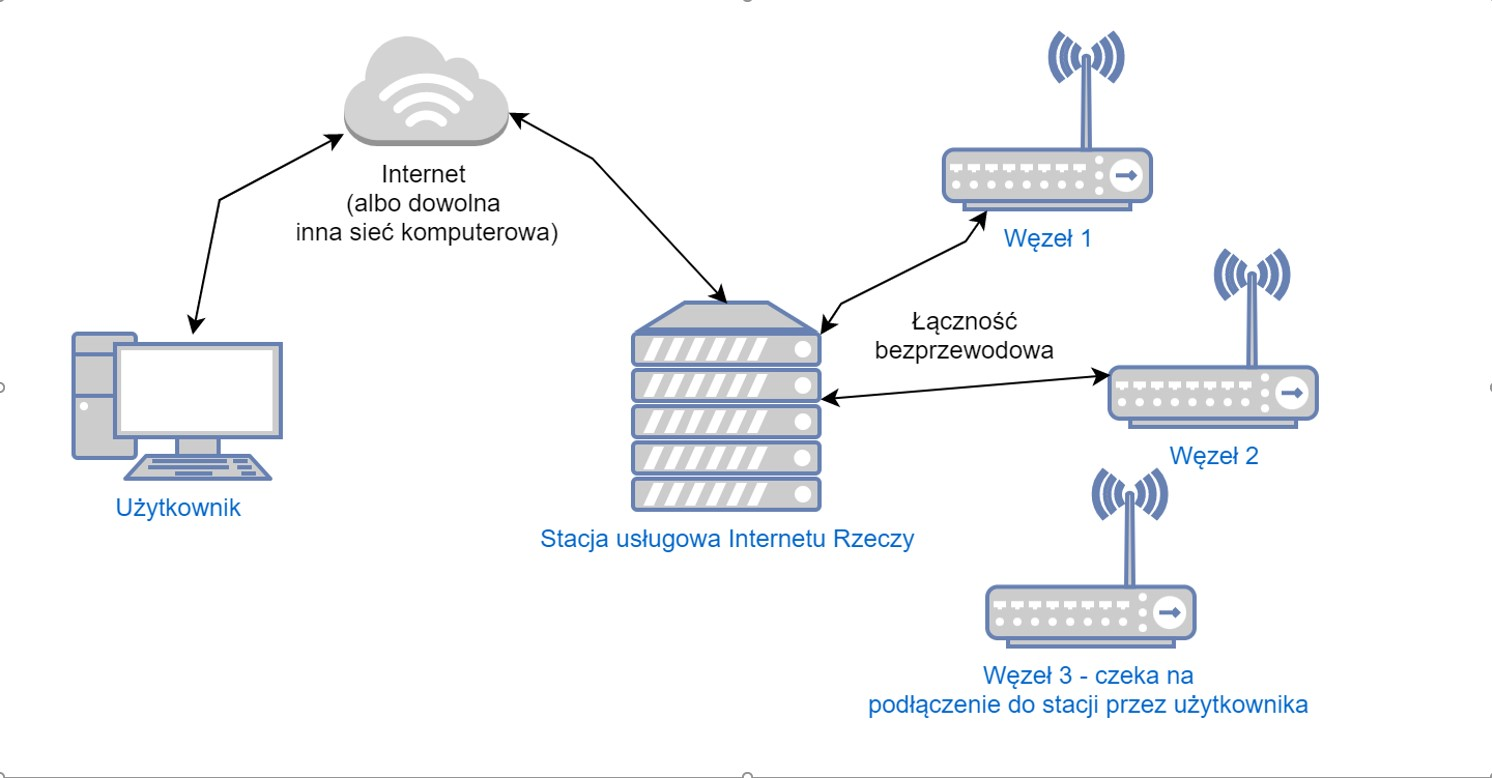
\includegraphics[scale=0.38]{zalozenia}
\caption{Schemat blokowy systemu IoT z dedykowaną stacją usługową}
\end{figure}

%----4------
\chapter{Dobór technologii}

Na podstawie założeń z poprzedniego rozdziału wyróżniono trzy główne zadania:
\begin{itemize}
\item konstrukcja stacji,
\item	konstrukcja węzła sieci,
\item	opracowanie protokołu komunikacyjnego. 
\end{itemize}
Pracę nad każdym z powyższych punktów rozpoczęto od odpracowania stosu technologicznego w postaci sprzętu, języka programowania i pozostałych niezbędnych narzędzi, które posłużą do realizacji.

%----4.1------
\section{Stacja usługowa}

Projekt stacji usługowej która ma za zadanie pełnić funkcje serwera, oraz gromadzić i przetwarzać dane, zakłada stworzenie oprogramowania i uruchomienie go na komputerze.  Z tego powodu do jej konstrukcji trzeba wykorzystać zarówno odpowiednie oprogramowanie jak i sprzęt które będą optymalne z punktu widzenia potrzeb projektu. 

%----4.1.1.------
\subsection{Sprzęt}
Na wstępie warto wytłumaczyć rzecz zawartą bezpośrednio w temacie pracy, czyli wykorzystanie komputera jednopłytkowego do konstrukcji stacji. Teoretycznie w tym celu sprawdziłby się każdy komputer osobisty, lecz byłoby to marnotrawienie jego faktycznych możliwości oraz zużycie energii i koszt samego urządzenia byłyby nieproporcjonalnie duże do złożoności zadania. O wiele lepszym rozwiązaniem jest zastosowanie komputera jednopłytkowego, który charakteryzuje się wielokrotnie mniejszą ceną i poborem prądu oraz wymiarami w porównaniu do zwykłych komputerów.
\par
W przypadku stacji należy wybrać sprzęt o odpowiedniej ilości zasobów tak aby możliwe było uruchomienie na nim wysokopoziomowego oprogramowania, które będzie pełnić rolę serwera. Samo urządzenie powinno wspierać najpopularniejsze protokoły komunikacyjne oraz mieć możliwość rozbudowy pamięci ze względu na potencjalnie dużą ilość gromadzonych danych. Poniżej przedstawiono kilka spośród najpopularniejszych modeli komputerów jednopłytkowych dostępnych na rynku:
\begin{itemize}
\item	Raspberry Pi 4 B - komputer z centralną jednostką obliczeniową Broadcom BCM2711 wyposażoną w 4 rdzenie procesora o 64 bitowej architekturze ARM Cortex-A53 pracujący z częstotliwością taktowania 1,5 GHz. W połączeniu z nawet 8 GB wbudowanej pamięci ram jest to wystarczająca ilość zasobów, aby uruchomić na komputerze dedykowany system operacyjny z graficznym interfejsem użytkownika oparty na jądrze systemu Linux. Z urządzenia można korzystać tak z komputera osobistego przy użyciu bezpośrednio podłączonych urządzeń peryferyjnych, lecz w celu oszczędzania zasobów rekomendowane jest stosowanie systemu operacyjnego bez graficznej powłoki i obsługa poprzez zdalną sesje wiersza poleceń. Raspberry Pi 4b posiada między innymi 40 pinów GPIO, porty USB, gniazdo Ethernet, wejście HDMI, Bluetooth i Wi-Fi. Moc urządzenia wynosi około 4W, ale przy większym obciążeniu procesora może się okazać, że potrzebne jest dodatkowe aktywne chłodzenie, które zwiększy zapotrzebowanie na energie.  
\item	Raspberry Pi Zero WH – uboższa wersja pod względem ilości zasobów sprzętowych powyższego komputera. Charakteryzuje się częstotliwością taktowania procesora wynoszącą 1 GHz, zaledwie 512 MB wbudowanej pamięci RAM i 1 rdzeniowym procesorem. Relatywnie gorsze parametry przekładają się na niższą cenę, zużycie energii oraz wymiary, co sprawa, że Raspberry Pi Zero jest przeznaczone do mniej wymagających zastosowań.
\item	Intel NUC – seria wydajnych minikomputerów wyposażona w funkcje do obsługi multimediów gier oraz pracy. Urządzenia z tej gamy posiadają procesory Intel w architekturze x86 wraz z wbudowaną kartą graficzną i obsługują do 32 GB pamięci RAM. Powyższa specyfikacja niczym nie odbiega od współczesnych komputerów dlatego można powiedzieć, że jest to sprzęt przeznaczony do bezpośredniego korzystania przez użytkownika, a nie do zastosowania w Internecie Rzeczy.
\end{itemize}
\begin{table}[H]
\centering
\begin{tabular}{|l|l|l|l|}
\hline
SBC          & Raspberry Pi model 4 b & Raspberry Pi Zero WH & Intel NUC        \\ \hline
Moc          & 6,25W                  & 0,9W                 & 90W              \\ \hline
Procesor     & ARM, 4 rdzenie         & ARM, 1 rdzeń         & x86, 4 rdzenie   \\ \hline
Taktowanie   & 1,5GHz                 & 1GHz                 & od 2,7 do 4,5GHz \\ \hline
Pamięć RAM   & od 2 do 8GB            & 512mB                & do 32GB          \\ \hline
GPIO         & 40 pinów               & 40 pinów             & Brak             \\ \hline
I2C/SPI/UART & Tak                    & Tak                  & Nie              \\ \hline
Ethernet     & Tak                    & Nie                  & Tak              \\ \hline
Cena         & ≈300zł                 & ≈60zł                & ≈1500zł          \\ \hline
\end{tabular}
\caption{Porównanie parametrów opisywanych komputerów jednopłytkowych}
\end{table}
\par
Spośród powyższych modeli wybrano Raspberry Pi 4 model b z dwoma giga bajtami pamięci RAM. Wszystkie jego właściwości wraz z przystępną sprawiają, że świetnie nadaje się do wykorzystania w projekcie. Raspberry Pi Zero nie posiada istotnych zalet, które by rekompensowały gorsze parametry, z kolei Seria Intel NUC jak już wcześniej wykazano nie nadaje się do IoT.
\begin{figure}[H]
\centering
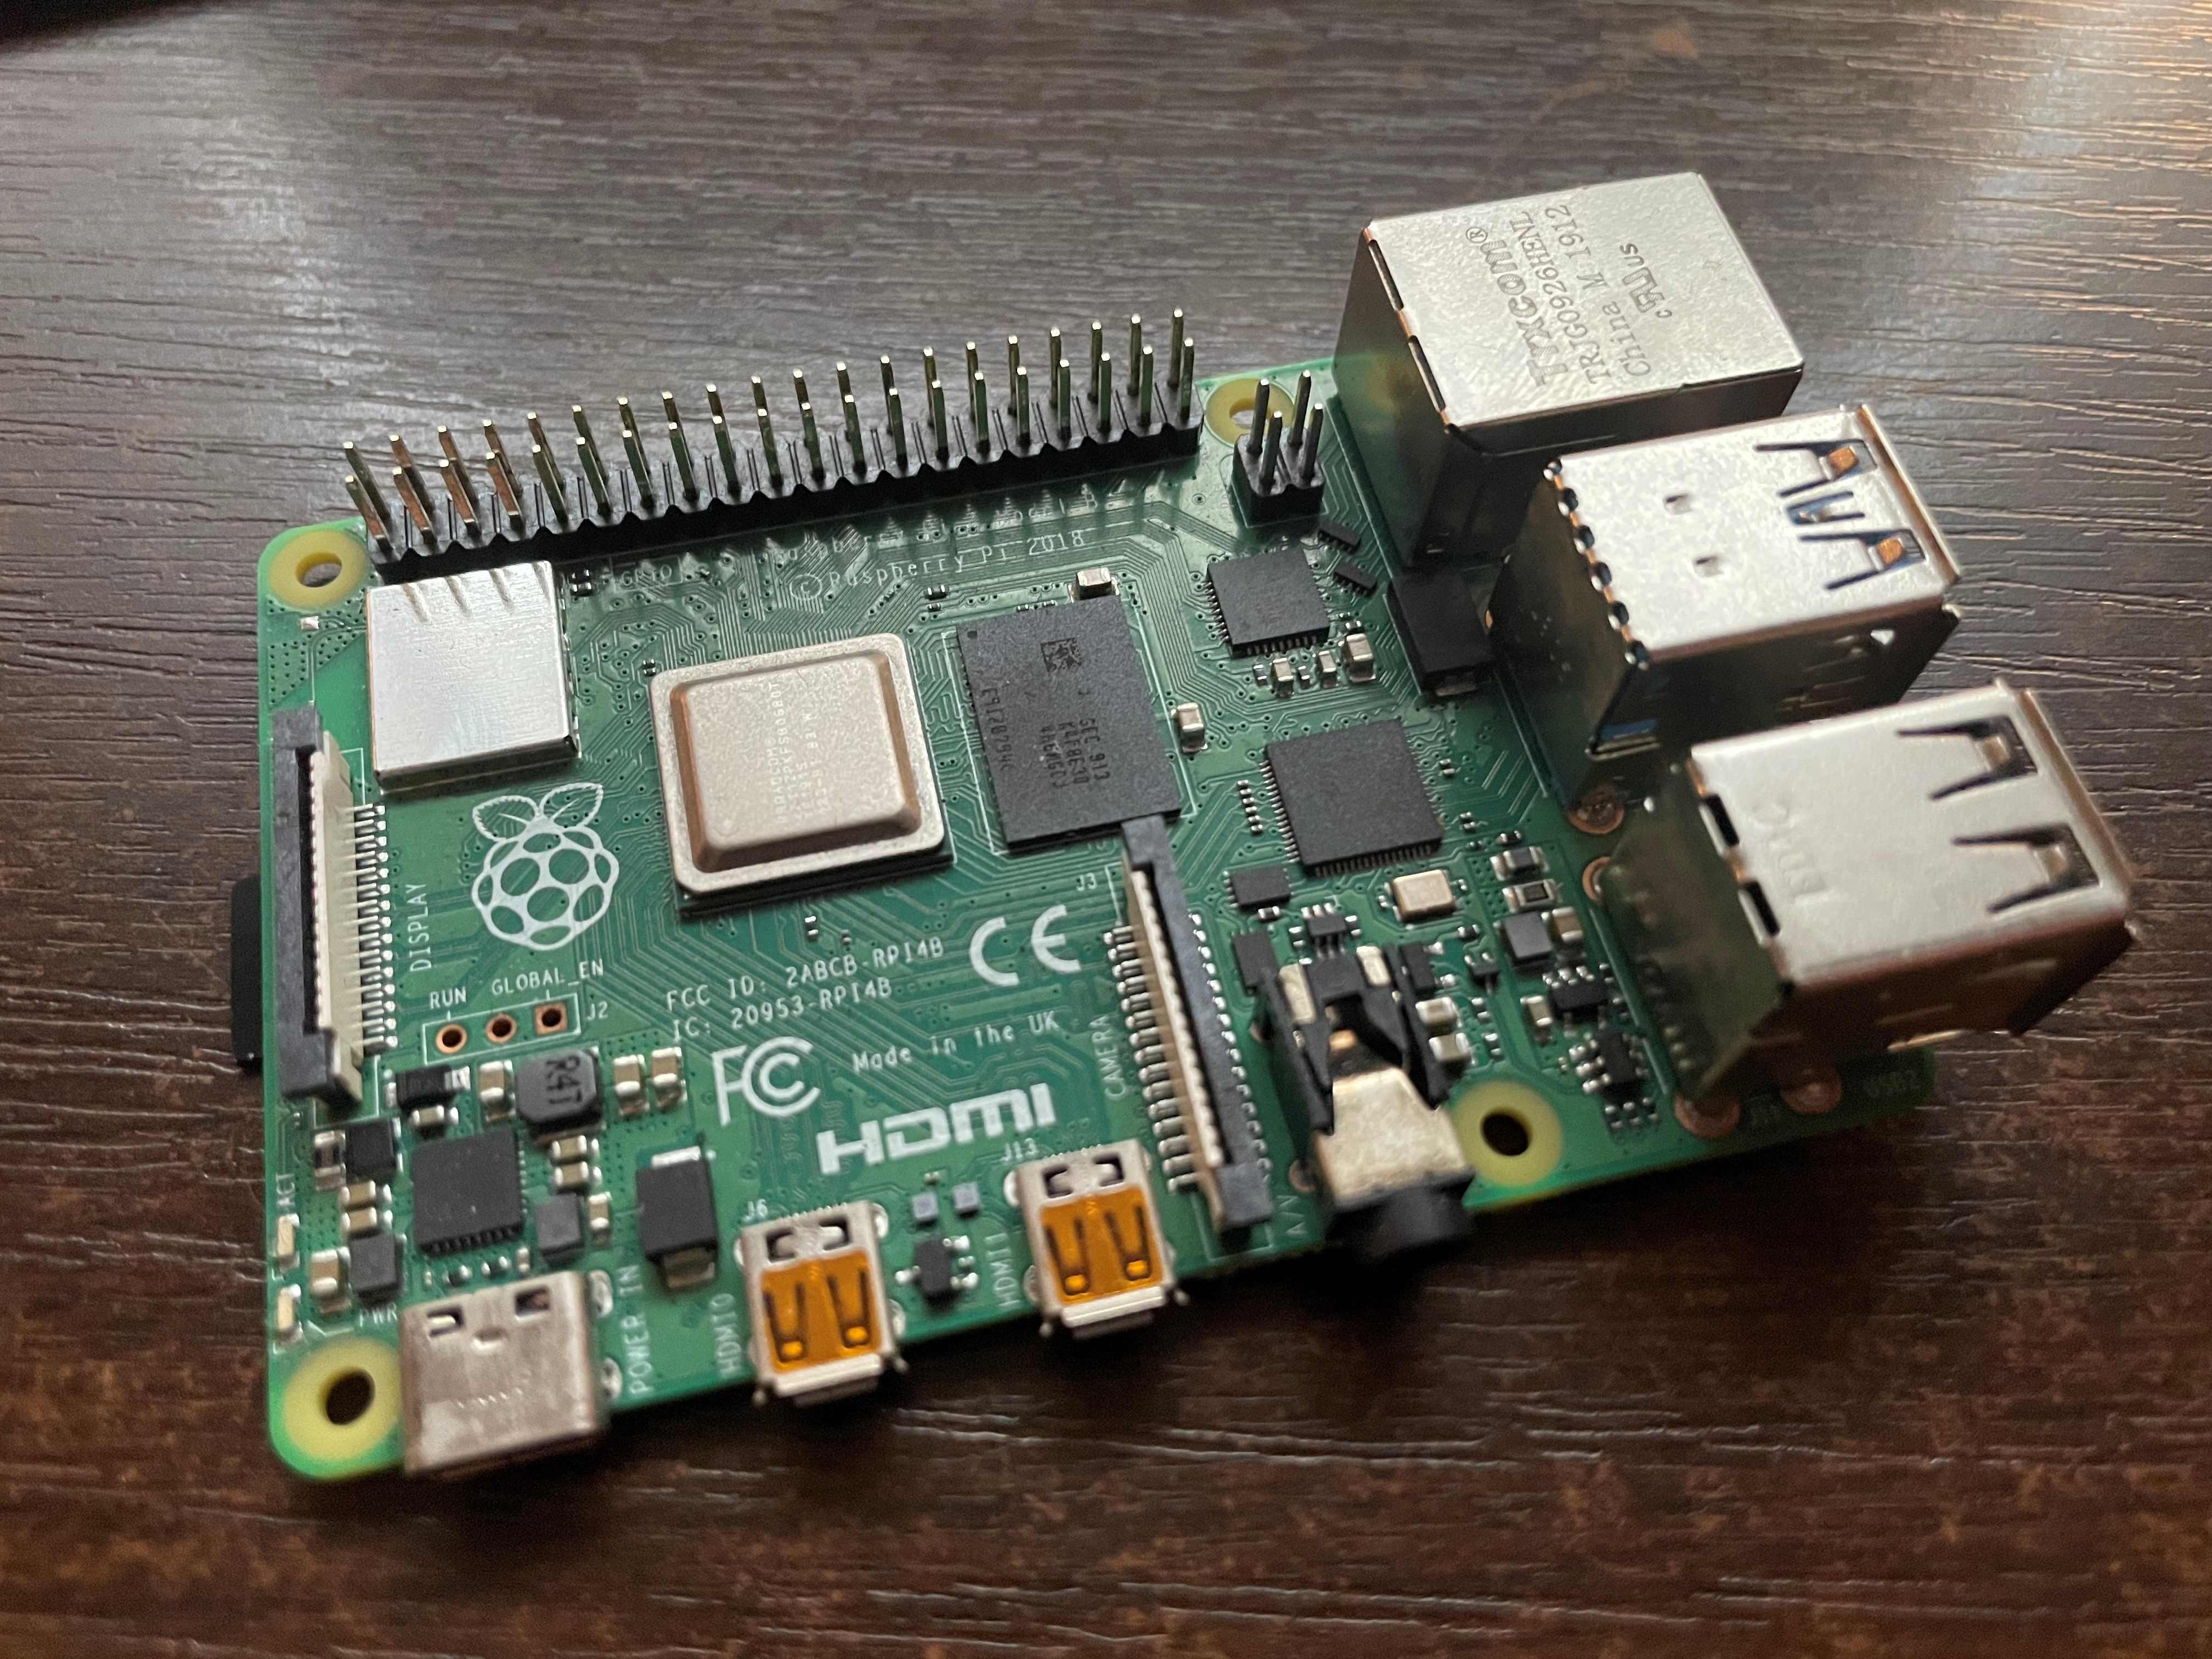
\includegraphics[scale=0.12]{rpi}
\caption{Komputer jednopłtykowy Raspberry Pi model 4b użyty do konstrukcji stacji usługowej}
\end{figure}


%----4.1.2.------
\subsection{Oprogramowanie}
Po wyborze sprzętu należało wybrać oprogramowanie. Zgodnie ze schematem blokowym z rysunku 3.1 komputer jednopłytkowy ma komunikować się z komputerem użytkownika poprzez Internet.  Z tego stacja usługowa między innymi musi pełnić funkcję serwera WWW oraz potrzebuje oprogramowania, które przetworzy dane i pokaże je użytkownikowi, dlatego wybrano następujące technologie:

\begin{itemize}
\item Python 3.6 – język programowania 
\item Flask – biblioteka do stworzenia aplikacji internetowej 
\item SQLite – baza danych
\item Nginx – serwer WWW 
\item uWSGI – serwer aplikacji
\end{itemize}

\begin{figure}[H]
\centering
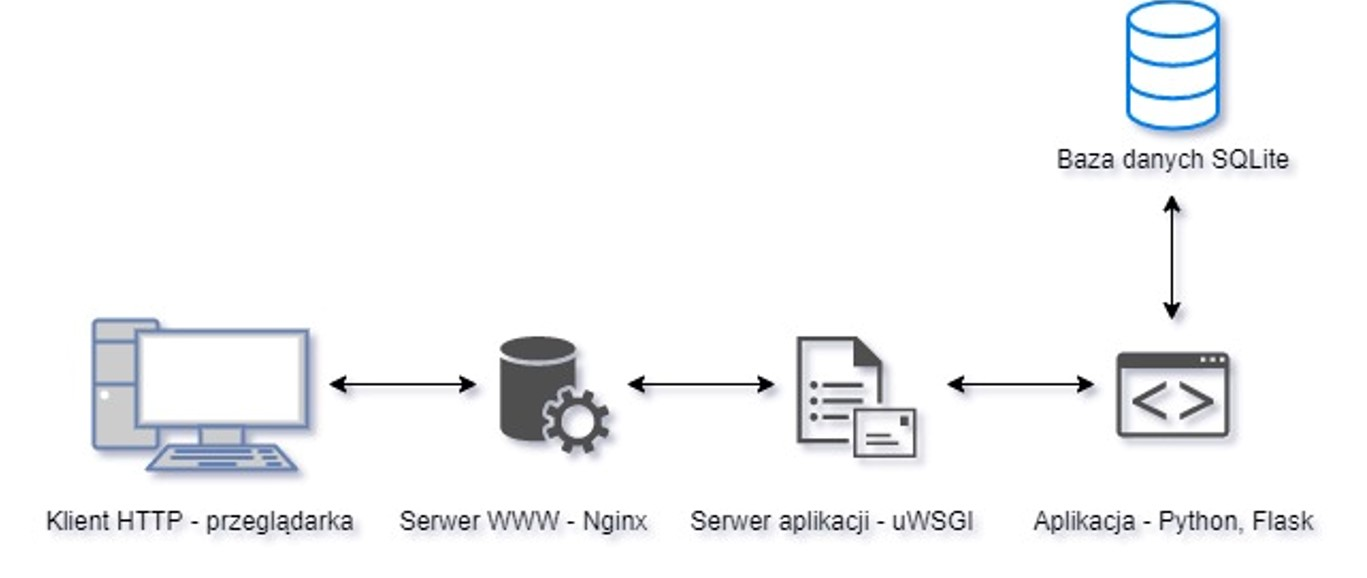
\includegraphics[scale=0.43]{stos}
\caption{Diagram stosu technologicznego stacji usługowej }
\end{figure}

\par
Wybór Python’a 3 jest dość oczywisty w przypadku chęci tworzenia aplikacji na Raspberry Pi. Jest on preinstalowany razem z systemem operacyjnym, posiada gotowe biblioteki do interakcji z pinami GPIO i powszechnie się go stosuje w niemal każdej dziedzinie programowania począwszy od tworzenia stron internetowych skończywszy na uczeniu maszynowym. 
\par
Istotnym elementem, o który trzeba zadbać jest przechowywanie danych pochodzących z czujników. Można by gromadzić je w surowych plikach tekstowych, lecz biorąc pod uwagę przewidywaną ilość danych nie jest to optymalne podejście. Z tego powodu należy zastosować relacyjną bazę danych opartą na standardzie SQL. Do zarządzania bazą zostanie wykorzystane otwarte oprogramowanie SQLite, które jest kompatybilne z Pythonem. 
\par
Z racji, że projekt zakłada stworzenie aplikacji Internetowej warto skorzystać z gotowej biblioteki, aby nie implementować od zera logiki odpowiedzialnej za kierowanie ruchem sieciowym i obsługę podstawowych żądań. W tym celu wybrano jedną z najpopularniejszych bibliotek do tworzenia aplikacji Internetowych, czyli Flask. Jest ona relatywnie prosta i „lekka”, przykładowa aplikacja typu „hello world”, która w tym przypadku ma za zadanie obsłużyć żądanie http typu GET i zwrócić krótki tekst zawiera dosłownie kilka linii kodu. Dodatkową jej zaletą jest elastyczność, skalowalność i możliwość dostosowania części składowych projektu do własnych potrzeb.
\par
Aby aplikacja była dostępna z poziomu przeglądarki potrzebny jest program, który obsłuży żądania protokołu http, czyli serwer WWW. Na potrzeby relatywnie prostego projektu każdy z popularnych programów dobrze sprawdzi się w tej roli dlatego ze względu na osobiste preferencje autora pracy wybrano Nginx. 
\par
Ostatnim elementem jest komunikacja serwera WWW samą aplikacją. Internetowe frameworki języka Python w tym celu korzystają z protokołu wsgi (ang.  Web Server Gateway Interface). Niestety Nginx nie obsługuje tego protokołu, dlatego wymagany jest program uWSGI pełniący funkcję serwera aplikacji. Przechwytuje on żądania http z serwera WWW i przekazuje je w akceptowalnej formie do aplikacji stworzonej w języku Python.
\par

%----4.2.------
\section{Węzeł}

Konstrukcja węzła sieci nie jest bezpośrednio tematem pracy, ale jeśli zależy nam na bezpieczeństwie musi podlegać on pewnym standardom. Informacje wysyłane w przestrzeń przez węzeł powinny być możliwe do odczytania tylko przez stacje która została z nim sparowana.
\par
Do konstrukcji mógłby posłużyć drugi komputer jednopłytkowy, lecz wymagania sprzętowe nie są tak wygórowane jak w przypadku stacji. Z tego powodu zdecydowano się na wykorzystanie mikrokontrolera, który jest znacząco tańszy i charakteryzuje się mniejszym poborem prądu. Wybór padł na prawdopodobnie najpopularniejszą platformę programistyczną dla systemów wbudowanych, czyli Arduino UNO. Wspomniany moduł posiada mikrokontroler ATmega238P oparty o 8 bitową architekturę AVR taktowany zegarem o częstotliwości 16 MHz. Urządzenie posiada 2 KB pamięci SRAM oraz 32 KB flash. Układ wyposażono w 14 cyfrowych wyjść obsługujących najpopularniejsze interfejsy komunikacyjne oraz przetwornik analogowo-cyfrowy, a całość można programować w języku C++. 

%----4.2.------
\section{Protokół komunikacyjny}

Ostatnim elementem całości jest protokół komunikacyjny. Na wstępie założono, że komunikacja jest bezprzewodowa dlatego oczywiste jest, że będzie odbywać się poprzez fale radiowe. Na rynku obecnych jest przynajmniej kilkanaście technologii bezprzewodowej transmisji z czego każda posiada inne parametry takie jak zasięg, szybkość transmisji czy pobór prądu. 
\par
Z racji, iż stacja nie ma konkretnego zastosowania oznacza to, że nie jest powiedziane w jakich warunkach będzie pracować. Z tego powodu przyjęto najprostszy przypadek, czyli węzły sieci znajdują się w odległości maksymalnie kilku metrów od stacji, są zasilane z sieci a ilość przesyłanych danych jest niewielka. Oznacza to, że na wstępie można odrzucić wszystkie technologie charakteryzujące się niskim poborem prądu bądź dużą szybkością transmisji.
\par
Po zawężeniu obszaru poszukiwań oczywistym wyborem w kwestii komunikacji staje się Bluetooth. Działa on w nielicencjonowanym paśmie ISM o częstotliwości 2.4 GHz [10] i szybkość transmisji wynosi 2.1 MB/s w trybie EDR (ang. Enchanced Data Rate).  Standard działa w architekturze „master-slave”, gdzie jeden węzeł typu „master” może na raz komunikować się z 7 węzłami typu „slave”. W najpowszechniejszej klasie mocy 2.5mW teoretyczny zasięg wynosi 10 metrów co w połączeniu z pozostałymi parametrami idealnie odpowiada na potrzeby projektu.
\par
Standard Bluetooth również posiada liczne profile, które służą do zapewnienia kompatybilności pomiędzy aplikacjami oraz urządzeniami. Istnieje kilkanaście profili stosowanych między innymi w bezprzewodowych zestawach słuchawkowych bądź do komunikacji z drukarką. W projekcie ograniczono się do jednego profilu określanego mianem wirtualnego portu szeregowego SPP (ang. Serial Port Profile). 
Po wybraniu protokołu należy się jeszcze upewnić, że zarówno węzeł jak i stacja będą z nim współpracować. O ile komputer jednopłytkowy Raspberry Pi posiada wbudowany moduł Bluetooth tak nie znajdziemy go w platformie programistycznej użytej do konstrukcji węzła. Z tego powodu potrzebny jest zewnętrzny moduł, w tym przypadku wybrano model powszechnie stosowany w amatorskich konstrukcjach, czyli HC-05. Moduł komunikuje się poprzez interfejs szeregowy UART, moc jego nadajnika wynosi 2.5mW i posiada wcześniej wymieniony profil SPP.

\begin{figure}[H]
\centering
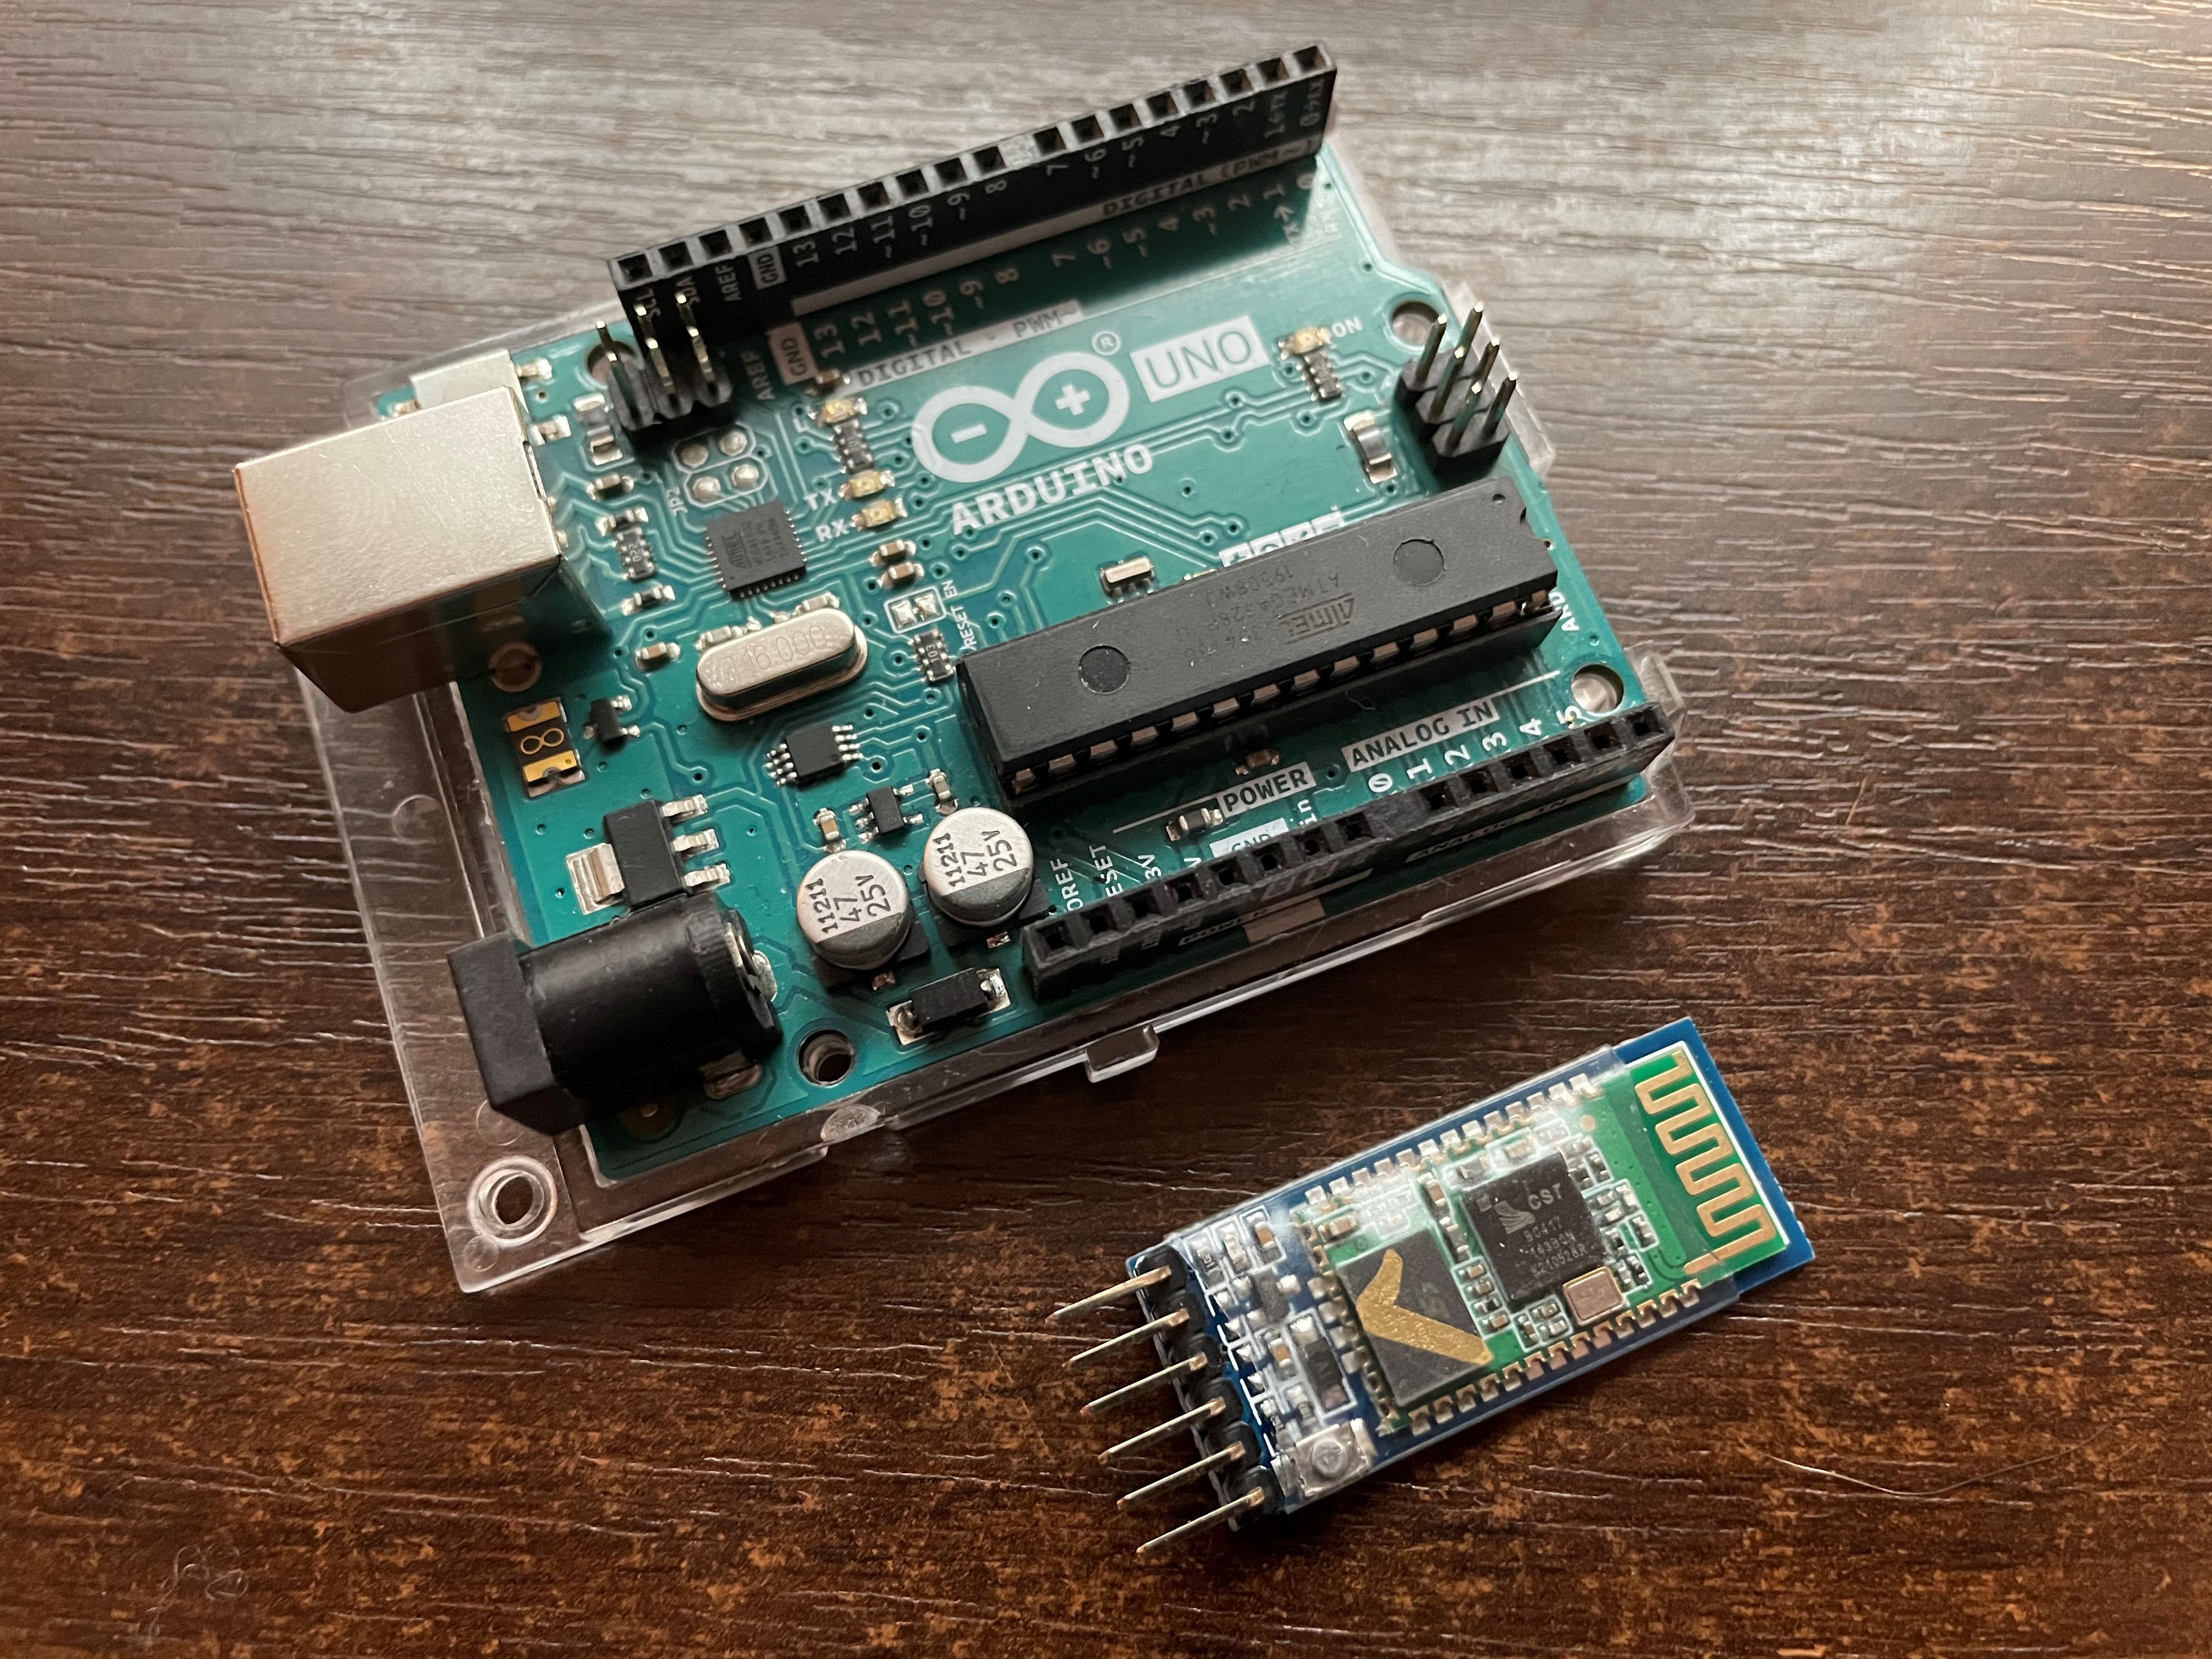
\includegraphics[scale=0.12]{hc05}
\caption{Elementy, które posłużyły do konstrukcji węzła, Arduino UNO i moduł Bluetooth HC-05}
\end{figure}

%----5-----
\chapter{Realizacja stacji usługowej}

%----5.1.-----
\section{Aplikacja internetowa}

Realizacje rozpoczęto od konfiguracji komputera jedno płytkowego poprzez zainstalowanie systemu operacyjnego Raspberry Pi OS oraz pozostałego oprogramowania i bibliotek wymienionych w stosie technologicznym stacji usługowej. Dodatkowo podłączono komputer do sieci LAN poprzez Wi-Fi, aby umożliwić wygodną pracę zdalną z komputera osobistego za pośrednictwem protokołu SSH. Kolejnym krokiem było stworzenie szkieletu samej aplikacji, co dzięki bibliotece Flask okazało się być niezwykle proste. Cała logika odpowiedzialna za obsługę żądań przychodzących z serwera aplikacji zawarta jest w jednym pliku i została przedstwiona we fragmencie kodu 5.1.
\begin{algorithm}[H]
\centering
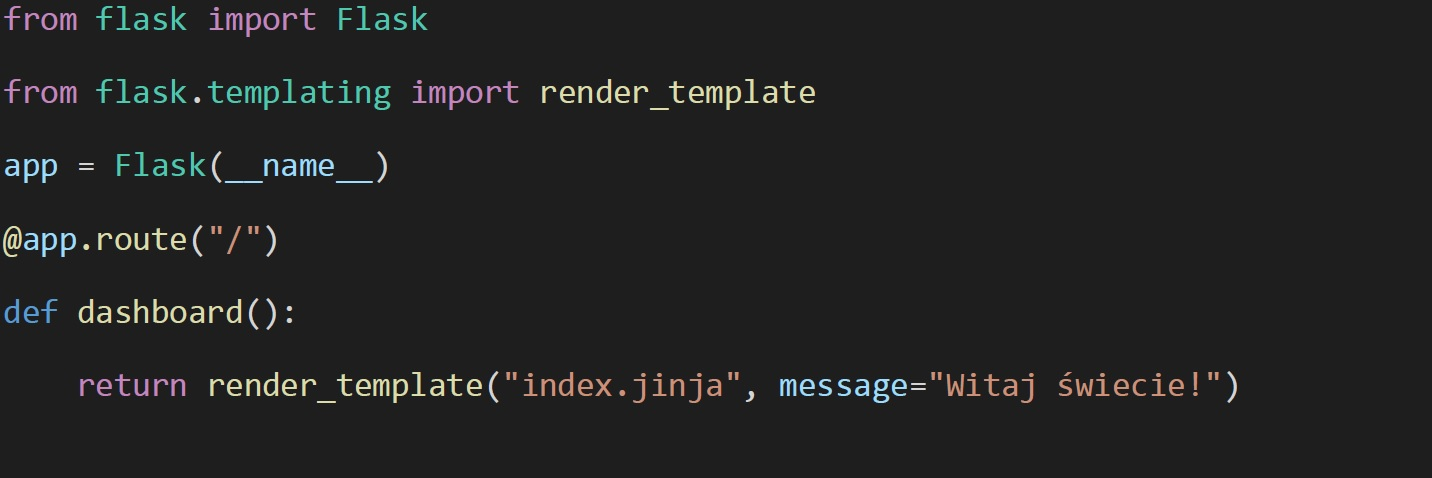
\includegraphics[scale=0.42]{kod}
\caption{Fragment odpowiedzialny za obsługę żądań przychodzących z serwera}
\end{algorithm}

\begin{algorithm}[H]
\centering
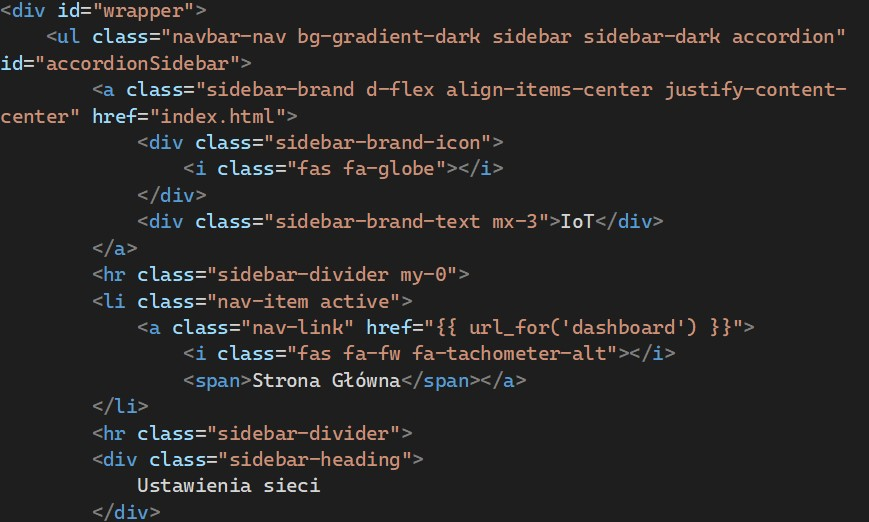
\includegraphics[scale=0.7]{kod_html}
\caption{Fragment kodu użytego szablonu HTML}
\end{algorithm}

Powyższy kod sprawia, że aplikacja po otrzymaniu żądania typu GET od serwera aplikacji zwróci kod strony zawarty w pliku „index.jinja” wraz z dynamicznie dodaną wiadomością „Witaj świecie!”. Sama treści strony została stworzona na podstawie darmowego szablonu HTML dostępnego w Internecie, którego fragment przedstawiono w kodzie 5.2.  Aby przetestować, czy całość działa wystarczy wpisać w przeglądarkę adres IP stacji który został przydzielony przez router. Poniżej przedstawiono rezultat:
\begin{figure}[H]
\centering
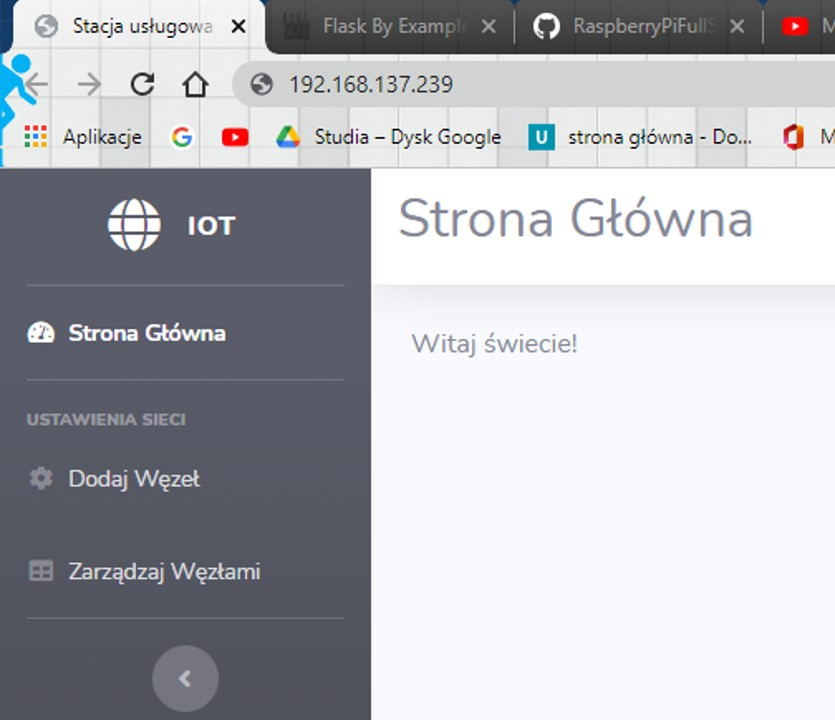
\includegraphics[scale=0.6]{szkielet}
\caption{Zrzut ekranu działającego szkieletu aplikacji}
\end{figure}


%----5.2.-----
\section{Baza danych}
Kolejnym krokiem było zaimplementowanie funkcjonalności wymienionych w założeniach. Z racji, iż aplikacja przede wszystkim ma zbierać i przetwarzać informacje prace rozpoczęto od projektu bazy danych. 
\begin{figure}[H]
\centering
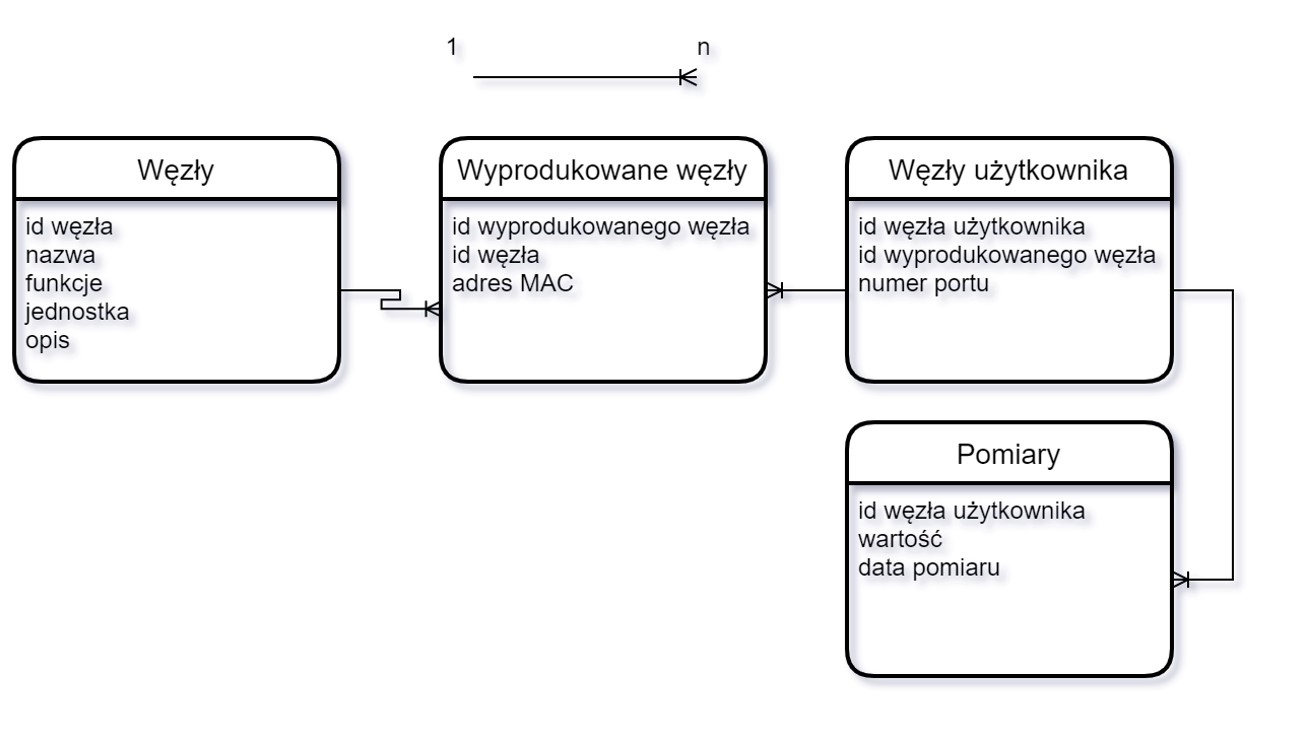
\includegraphics[scale=0.5]{db}
\caption{Szkic bazy danych}
\end{figure}
\par
Na rysunku 5.2. przedstawiono logiczny model bazy danych który posłużył później do implementacji. Wszystkie relacje należy rozumieć jako „jeden do wielu” gdzie linia zakończona rozwidleniem oznacza, że w danej tabeli występuje wielokrotnie rekord z innej tabeli będącej z nią w relacji. \par
W zaproponowanym modelu tabela „Węzły” zawiera w sobie listę wszystkich rodzajów węzłów. Może być to dowolny czujnik temperatury, albo zdalnie sterowany przekaźnik. Przykładowo we fragmencie kodu 5.2. wstawiono do tej tabeli węzeł o nazwie „Węzeł testowy” z zadaną listą funkcji.  \par
Tabela „Wyprodukowane węzły” reprezentuje fizyczne, wyprodukowane węzły sieci. Oznacza to, że każdy taki węzeł posiada unikalną kombinacje swojego własnego identyfikatora, identyfikatora rodzaju oraz adresu MAC. Dzięki temu użytkownik podając numer konkretnego węzła będzie mógł dodać go do sieci, z kolei aplikacja będzie wiedziała jak z nim „rozmawiać”. W tym momencie możliwe jest wyprodukowanie dowolnej ilości urządzeń, które stacja będzie postrzegać jako „Węzeł testowy” lecz każde z nich będzie miało swoją unikalną tożsamość.
Proponowana architektura również ma na celu skalowalność, dzięki czemu dodanie nowego rodzaju węzła o nowych, dotychczas nieznanych funkcjach nie będzie stanowić problemu i wymaga jedynie utworzenia odpowiedniego rekordu w tabeli „Węzły”. Ponad to zapewnia ona prywatność, ponieważ każdy wyprodukowany węzeł musi zostać wcześniej otrzymać unikalny identyfikator od producenta, więc nie będzie możliwe korzystanie z urządzeń wyprodukowanych przez osoby trzecie, które mogłyby nie spełniać standardów bezpieczeństwa. Co więcej cały plik bazy danych jest przechowywany w pamięci komputera jednopłytkowego więc tylko użytkownik ma dostęp do gromadzonych danych.
Kod 5.3. przedstawia fragment skryptu odpowiedzialnego za stworzenie całej bazy danych. W pierwszej kolejności nawiązywane jest połączenie z pustą bazą danych, po czym wykonywane są polecenia napisane zgodnie ze standardem SQL. Polecenie na poniższym listingu tworzy tabele o nazwie „nodes” odpowiadającej tabeli „węzły” z rysunku 5.2. i umieszcza w niej jeden testowy rekord o nazwie „Węzeł testowy”.
\par

\begin{algorithm}[H]
\centering
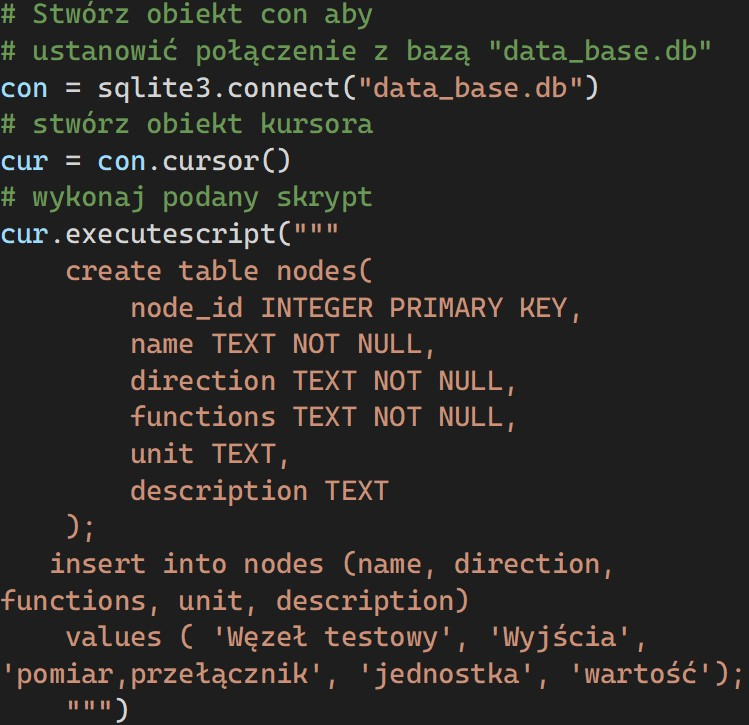
\includegraphics[scale=0.7]{kod_migracja}
\caption{Fragment skryptu odpowiedzialnego za tworzenie bazy danych}
\end{algorithm}

%----5.3.-----
\section{Łączność bezprzewodowa}
Ostatnim elementem oprogramowania stacji usługowej było zapewnienie łączności bezprzewodowej z węzłami przy użyciu Bluetooth. Schemat blokowy algorytmu służącego do nawiązania takiej łączności przedstawiono poniżej:
\begin{figure}[H]
\centering
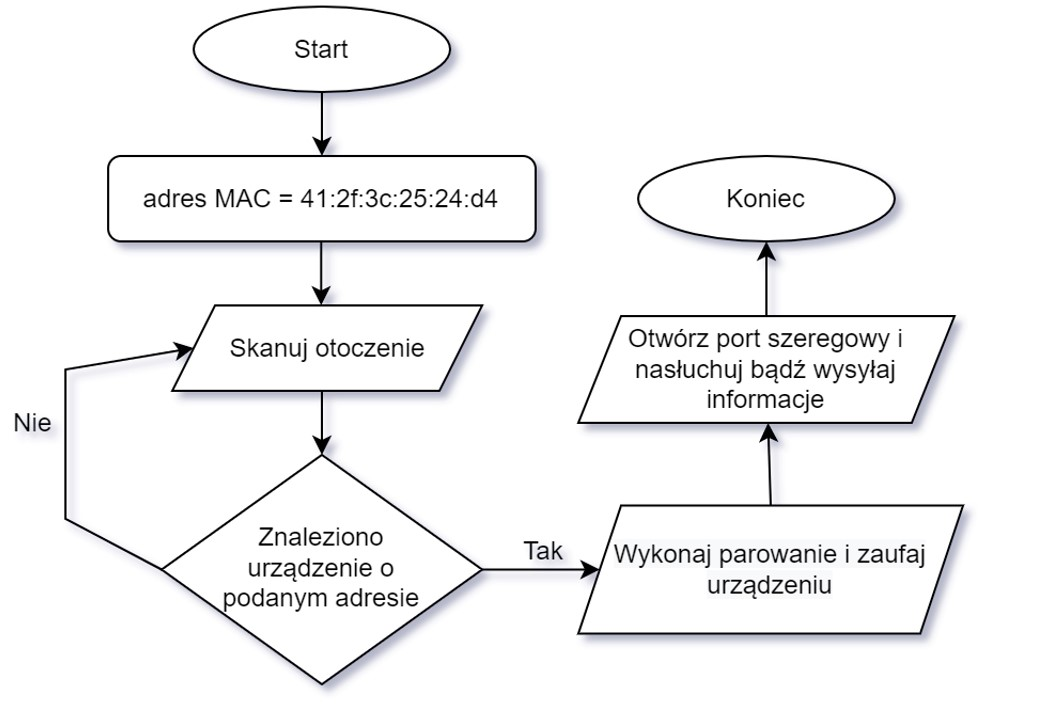
\includegraphics[scale=0.5]{algorytm}
\caption{Schemat blokowy algorytmu do nawiązywania łączności bezprzewodowej poprzez\,Bluetooth}
\end{figure}
\par
Na wstępnie musimy znać adres MAC modułu Bluetooth z którym chcemy się porozumieć. Kolejnym krokiem jest skanujemy otoczenie aż do skutku po czym należy wykonać procedurę parowania i zaufać urządzeniu. Po wykonaniu tych czynności pozostaje otworzyć port szeregowy i można wysyłać bądź odbierać informacje od modułu Bluetooth. Wszystkie powyższe operacje są implementowane przez system operacyjny i dostępne za pośrednictwem komend terminala systemu Linux więc autor pracy stworzył skrypt w języku Python który cały ten proces automatyzuje. Przykładowy fragment kodu 5.4. przedstawia funkcję odpowiedzialną za wysłanie do wiersza poleceń komputera polecenia „scan on”, które uruchamia procedurę skanowania w poszukiwaniu wykrywalnych urządzeń Bluetooth.

\begin{algorithm}[H]
\centering
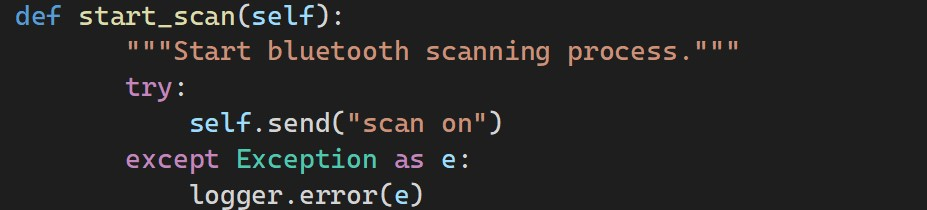
\includegraphics[scale=0.7]{kod_bt}
\caption{Fragment skryptu automatyzującego nawiązywanie łączności bezprzewodowej}
\end{algorithm}

%----5.4.-----
\section{Węzeł}
Ostatnim elementem projektu był węzeł sieci z którym stacja będzie się komunikować. Do konstrukcji węzła posłużyła platforma programistyczna dla systemów wbudowanych Arduino Uno zintegrowana z modułem Bluetooth HC-05. Schemat połączeń został przedstawiony na rysunku 5.5.

\begin{figure}[H]
\centering
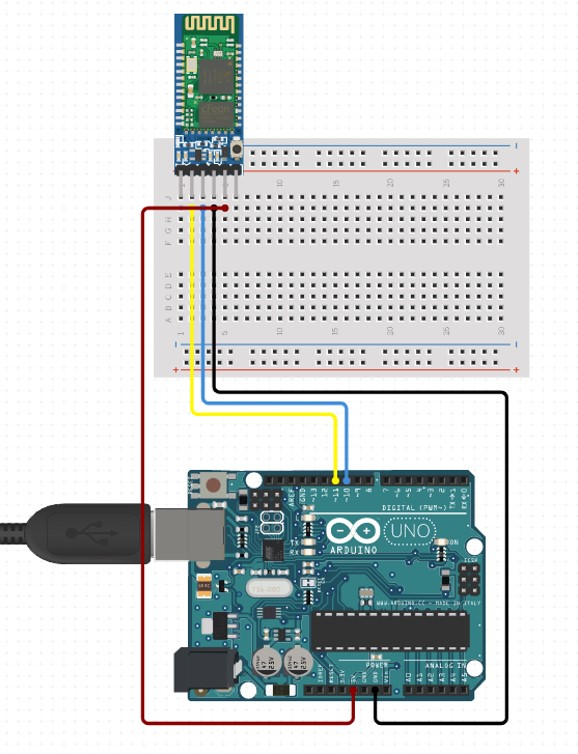
\includegraphics[scale=0.8]{schemat}
\caption{Schemat połączeń elektrycznych węzła sieci}
\end{figure}
\par
Moduł HC-05 komunikuje się poprzez interfejs szeregowy UART, więc wystarczy podłączyć jedynie wyprowadzenia służące do odbierania i wysyłania danych oraz masę i zasilanie. Mikrokontroler został zaprogramowany, aby wysyłać losowo generowaną liczbę co ma na celu symulować dokonywanie pomiaru za pośrednictwem zewnętrznego czujnika. Dodatkowo mikrokontroler w przypadku otrzymania odpowiedniej komendy zmieni stan jednego z wyjść cyfrowych które podłączone jest do wbudowanej w płytkę diody LED. Fragment kodu 5.5. przedstawia główną pętle programu mikrokontrolera. Docelowo zamiast diody do takiego wyjścia można podłączyć na przykład przekaźnik, który steruje urządzeniem zasilanym wysokim napięciem.

\begin{algorithm}[H]
\centering
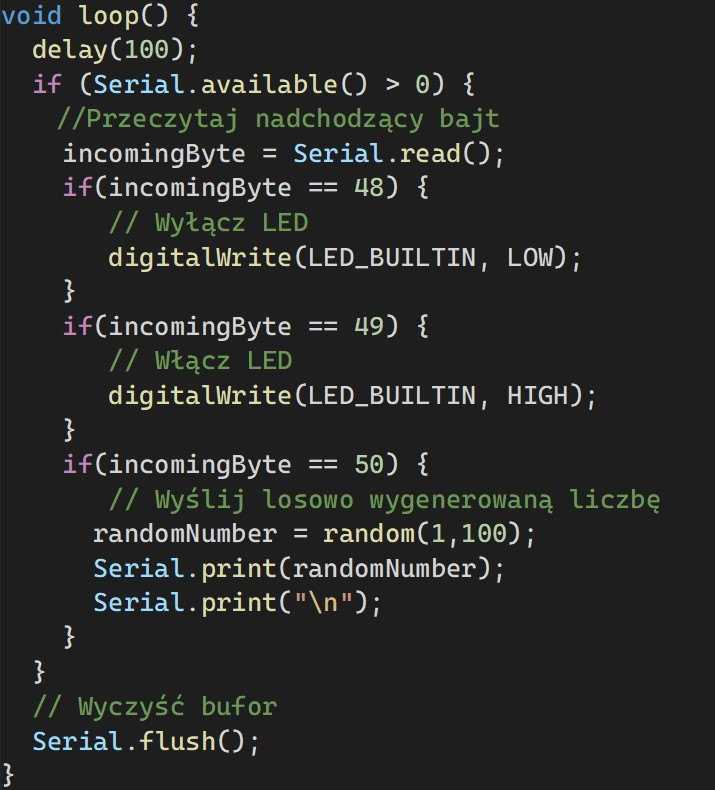
\includegraphics[scale=0.7]{kod_node}
\caption{Główna pętla programu mikrokontrolera}
\end{algorithm}

%----6.-----
\chapter{Testowanie}

%----6.1.-----
\section{Testy niezawodności łączności bezprzewodowej}
W ramach testów sprawdzono wpływ zakłócających sygnałów oraz przeszkód terenowych obecnych w mieszkaniu na niezawodność łączności bezprzewodowej przy użyciu standardu Bluetooth. W tym celu nadano 10000 ramek danych z w odstępach czasowych wynoszącym 1 ms i zbadano następujące parametry:

\begin{itemize}
\item Czas transmisji – różnica czasu pomiędzy ostatnią a pierwszą odebraną ramką \[ t = t_{koniec} - t_{start} \; \; \;  (6.1.)\]
\item	Sprawność transmisji – stosunek liczby poprawnie odebranych do ilości wszystkich wysłanych ramek\[ S = \frac{N_{odebranych}}{N_{wyslanych}} \; \; \;  (6.2.)\]
\item	Średnia arytemtyczna mocy odbieranego sygnału wyrażona w dBm wyliczona z pięciu pomiarów
\end{itemize}

%----6.1.1-----
\subsection{Układ pomiarowy}
Do pomiaru mocy odbieranego sygnału standardu Bluetooth użyto aplikacji „bluetooth scanner” dostępnej na telefonach z systemem operacyjnym android. Urządzeniem wykorzystanym do pomiarów był smartfon Samsung Galaxy A3 2016 wykorzystujący standard Bluetooth 4.0 w drugiej klasie mocy wynoszącej 2.5mW.
\par
W celu wyznaczenia niepewności pomiaru wykorzystano metodę statystyczną, polegającą na dokonaniu obliczeń na podstawie wielokrotnych pomiarów. Obliczona w ten sposób niepewność odpowiada odchyleniu standardowemu średniej z dokonanych pomiarów i jest określona wzorem  6.3.
\[ u(x) = \sqrt{ \frac{ \sum_{i=1}^{n} (x_i -x_{srednia}^2) } { n(n-1)  }}  \; \; \;  (6.3.)\]
\par
Gdzie: \par
 x\textsubscript{i}  - wynik pomiaru nr i 
\par
 x\textsubscript{średnia}  - średnia arytemtyczna ze wszystkich pomiarów
\par
 n - liczba pomiarów
\par

Za nadajnik sygnału posłużył węzeł sieci wykonany w ramach niniejszego projektu. Jest on wyposażony w moduł Bluetooth HC-05 działający w standardzie Bluetooth 2.0 i w drugiej klasie mocy 2,5mW [22]. \par
Odbiornikiem była stacja również uprzednio skonstruowana stacja usługowa Internetu Rzeczy z zastosowaniem komputera jednopłytkowego Raspberry Pi model 4 b. Podobnie jak nadajnik pracuje ona w klasie mocy 2,5mW lecz posiada standard Bluetooth w wersji 5.0 [23] \par
Wszystkie pomiary zostały przeprowadzone gdy smartfon był trzymany pionowo, tyłem do nadajnika, na wysokości około 50cm. Podczas mierzenia sprawności transmisji nadajnik pozostawał nieruchomy, a odbiornik zmieniał swoje położenie. Oba urządzenia znajdowały się na tej samej wysokości 50 cm nad ziemią. Cały układ pomiarowy został przedstawiony na rysunku 6.1.

\begin{figure}[H]
\centering
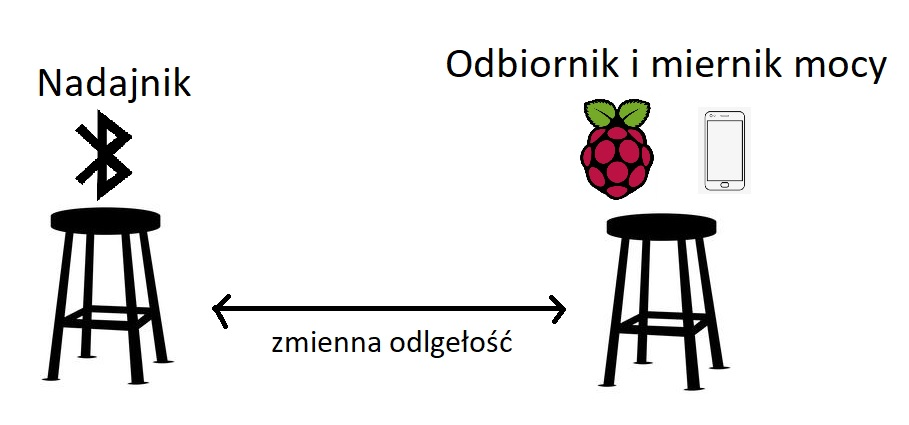
\includegraphics[scale=0.6]{uklad}
\caption{Schemat układu pomiarowego}
\end{figure}

%----6.1.2-----
\subsection{Środowisko testowe}
Testy przeprowadzono w dwóch różnych lokalizacjach. Pierwszą z nich jest mieszkanie w jednym z bloków mieszkalnych w Warszawie, schemat środowiska testowego przedstawiono na rysunku 6.2.
\begin{figure}[H]
\centering
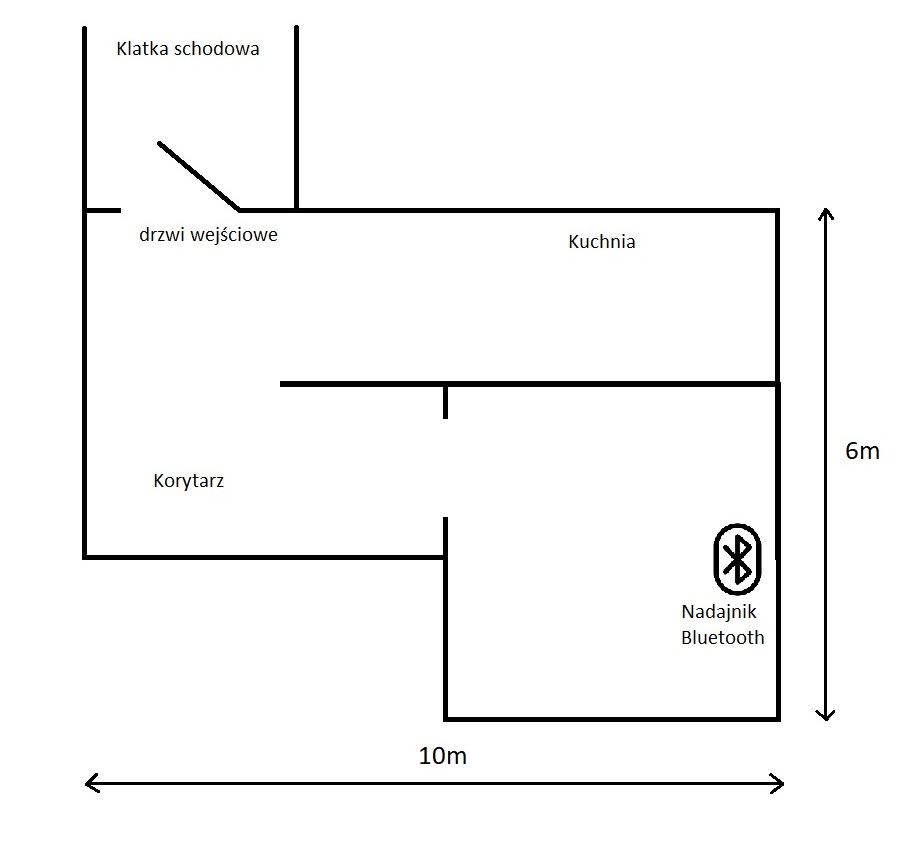
\includegraphics[scale=0.6]{mieszkanke}
\caption{Schemat środowiska testowego nr 1.}
\end{figure}
W otoczeniu obecnych jest wiele sieci Wi-Fi oraz Bluetooth, które potencjalnie utrudniają transmisje. W tabeli 6.1. i na rysunku 6.3. przedstawiono wyniki pomiarów mocy poszczególnych sygnałów w paśmie 2,4GHz przeprowadzonych w najbliższym otoczeniu nadajnika, zdecydowana większość z nich pochodzi od sąsiadów.
\begin{table}[H]
\centering
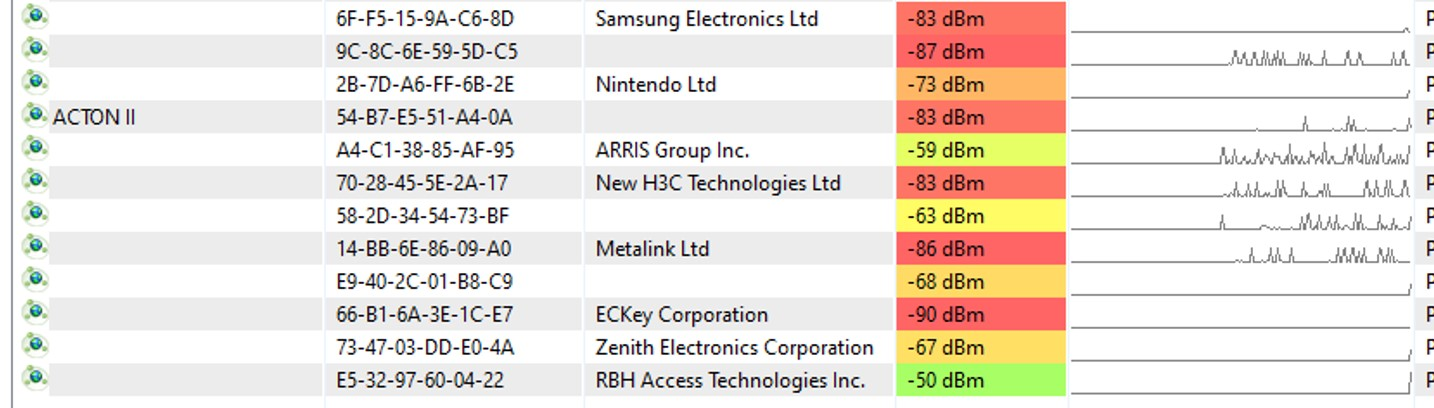
\includegraphics[scale=0.4]{bt}
\caption{Moce poszczególnych sygnałów Bluetooth w otoczeniu nadajnika w środowisku testowym nr 1.}
\end{table}
\begin{figure}[H]
\centering
\includegraphics[scale=0.35]{2,4Ghz}
\caption{Moce poszczególnych sygnałów Wi-Fi w otoczeniu nadajnika w środowisku testowym nr 1.}
\end{figure}
\par
Drugą lokalizacją jest jednorodzinny dom na prowincji. Na rysunku 6.4. został przedstawiony schemat środowiska testowego numer 2, budynek posiada dwie kondygnacje na których przeprowadzono pomiary – parter i pierwsze piętro. Czynnikami które uległy zmianie w porównaniu do środowiska numer 1 jest znacząco mniejsza ilość sygnałów Wi-Fi oraz Bluetooth. Na rysunku 6.6. widoczne są tylko dwie sieci z czego jedna z nich to prywatna sieć domowników, z kolei w tabeli 6.2. znajdują się tylko dwa sygnały pochodzące z bezprzewodowych urządzeń peryferyjnych.
\par
\begin{figure}[H]
\centering
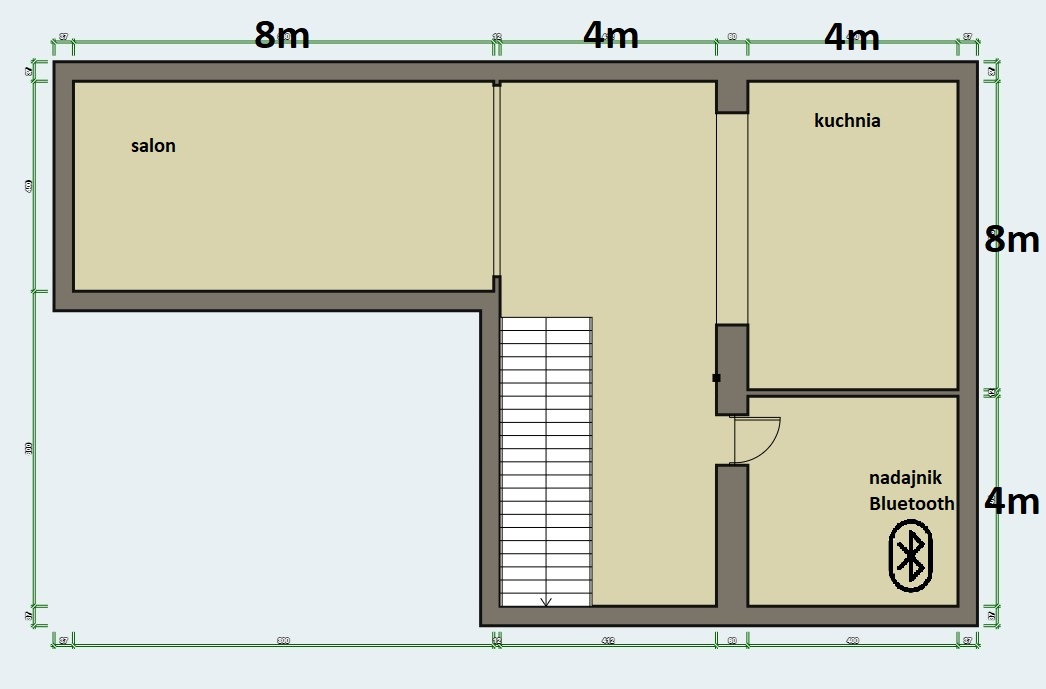
\includegraphics[scale=0.4]{dom1pietro}
\caption{Schemat środowiska testowego nr 2 - parter.}
\end{figure}
\begin{figure}[H]
\centering
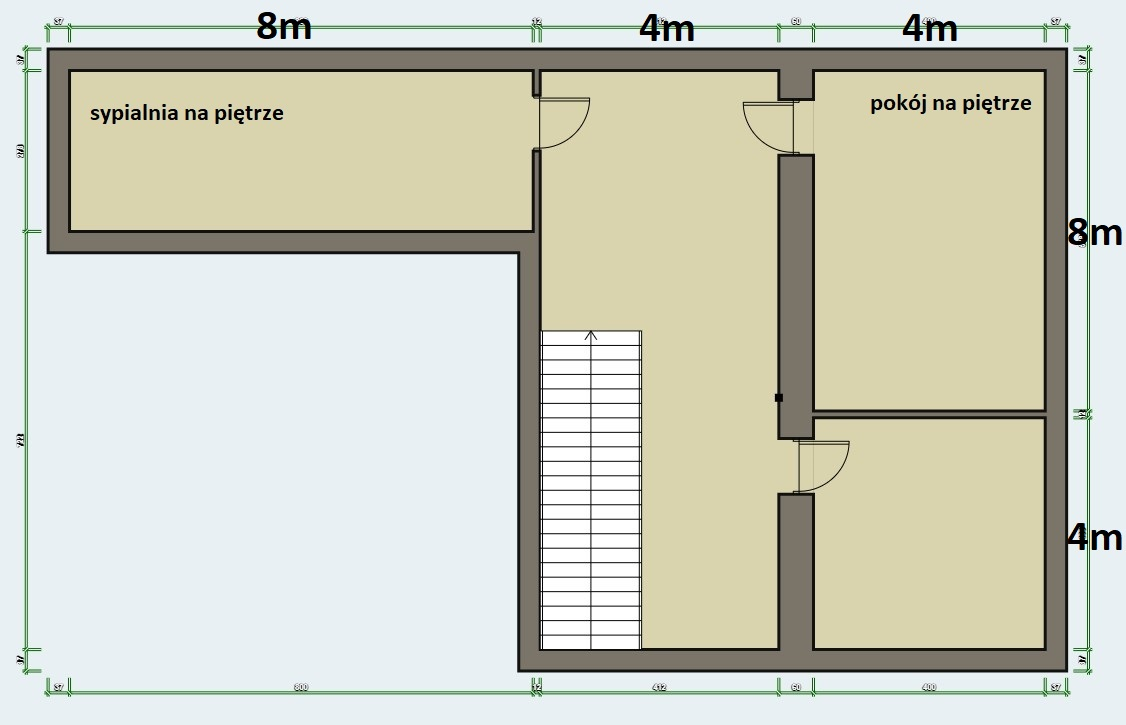
\includegraphics[scale=0.4]{dom2pietro}
\caption{Schemat środowiska testowego nr 2 - pierwsze piętro.}
\end{figure}
\begin{figure}[H]
\centering
\includegraphics[scale=0.35]{2,4Ghz_Dom}
\caption{Moce poszczególnych sygnałów Wi-Fi w otoczeniu nadajnika w środowisku testowym nr 2.}
\end{figure}
\begin{table}[H]
\centering
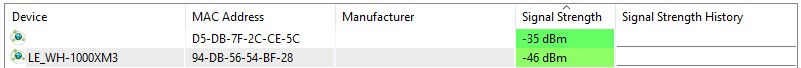
\includegraphics[scale=0.8]{bt_dom}
\caption{Moce poszczególnych sygnałów Bluetooth w otoczeniu nadajnika w środowisku testowym nr 2.}
\end{table}

%----6.1.2-----
\subsection{Pomiary}
W pierwszej kolejności w ramach próby kontrolnej przeprowadzono pomiary dla łączności przewodowej, a następnie powtórzono ten sam proces dla każdego wyszczególnionego na schemacie punktów. Wyniki dla środowiska testowego numer 1 przedstawiono w tabelach 6.3. i 6.4.
\begin{table}[H]
\begin{tabular}{|l|l|l|l|}
\hline
Miejsce                          & moc {[}dBm{]} & niepewność   {[}dBm{]} & odległość   od nadajnika {[}m{]} \\ \hline
obok nadajnika (przewód)         & n. d.         & n. d.                  & 0                                \\ \hline
obok nadajnika                   & -31,6           & 1,326649916            & 0                                \\ \hline
korytarz                         & -71,6           & 1,720465053            & 10                               \\ \hline
kuchnia                          & -62,6           & 1,630950643            & 3                                \\ \hline
drzwi wejściowe                  & -83,2           & 1,881488772            & 11,5                             \\ \hline
klatka schodowa, otwarte drzwi   & -86,8           & 1,356465997            & 12                               \\ \hline
klatka schodowa, zamknięte drzwi & ?             & ?                      & 12                               \\ \hline
\end{tabular}
\caption{Wyniki pomiarów mocy przeprowadzonych w środowisku testowym nr. 1}
\end{table}

\begin{table}[H]
\begin{tabular}{|l|l|l|}
\hline
Miejsce                          & czas transmisji {[}s{]} & sprawność transmisji {[}\%{]} \\ \hline
obok nadajnika (przewód)         & 50,805                  & 100                           \\ \hline
obok nadajnika                   & 50,781                  & 100                           \\ \hline
korytarz                         & 50,732                  & 100                           \\ \hline
kuchnia                          & 50,512                  & 100                           \\ \hline
drzwi wejściowe                  & 53,355                  & 100                           \\ \hline
klatka schodowa, otwarte drzwi   & 58.839                  & 90,8                          \\ \hline
klatka schodowa, zamknięte drzwi & -                       & 38,5                          \\ \hline
\end{tabular}
\caption{Wyniki pomiarów sprawności transmisji przeprowadzonych w środowisku testowym nr. 1}
\end{table}
\par
Pierwszą rzeczą, która można wywnioskować z powyższych pomiarów jest minimalna moc sygnału która zapewnia bezbłędną transmisję. Wynosi ona około -83 dBm i jest to wynik zgodny ze specyfikacją standardu Bluetooth według której minimalna moc mieści się w przedziale od -70 do -82 dBm.  Warto również zwrócić uwagę na to, że dla dostatecznie dobrego zasięgu czas transmisji pozostaje praktycznie taki sam jak w przypadku transmisji przewodowej. 
\par
Kolejną kwestią jest wpływ przeszkód i odległości na propagacje sygnału. Wyraźnie widać, że odległość 10 metrów w przypadku korytarza oraz ściana w przypadku kuchni nie wpływają na odbiór sygnału, zarówno czas jak i sprawność transmisji pozostają bez zmian. Dopiero przy drzwiach wejściowych, w odległości około 12 metrów od nadajnika obserwowalne stają się utrudnienia w postaci wydłużonego czasu nadawania. Poza obszarem mieszkania, na klatce schodowej można zaobserwować obniżenie sprawności transmisji do około 90\%. Zamknięcie drzwi wejściowych powoduje prawie całkowity zanik sygnału do tego stopnia, że transmisja zostaje w pewnym momencie bezpowrotnie przerwana, a moc odbieranego sygnału nie daje się zmierzyć przy użyciu wybranej metody, można jedynie szacować, że wynosi ona poniżej -90 dBm.
\par
Całą powyższą procedurę powtórzono dla środowiska testowego numer 2. Wyniki przedstawiono w tabelach 6.5. i 6.6.

\begin{table}[H]
\begin{tabular}{|l|l|l|l|}
\hline
Miejsce                    & moc {[}dBm{]} & niepewność   {[}dBm{]} & odległość   od nadajnika {[}m{]} \\ \hline
Obok   nadajnika (przewód) & n. d.         & n. d.                  & 0                                \\ \hline
Obok nadajnika             & -30,8         & 0,8                    & 0                                \\ \hline
Salon                      & -82           & 1,414213562            & 15                               \\ \hline
kuchnia                    & -75,8         & 1,280624847            & 10                               \\ \hline
Pokój na   piętrze         & -75,6         & 1,029563014            & 12                               \\ \hline
Sypialnia na   piętrze     & -84,6         & 1,326649916            & 18                               \\ \hline
\end{tabular}
\caption{Wyniki pomiarów mocy przeprowadzonych w środowisku testowym nr. 2}
\end{table}

\begin{table}[H]
\begin{tabular}{|l|l|l|}
\hline
Miejsce                    & czas transmisji {[}s{]} & sprawność transmisji {[}\%{]} \\ \hline
Obok   nadajnika (przewód) & 50.805                  & 100                           \\ \hline
Obok nadajnika             & 50.755                  & 100                           \\ \hline
Salon                      & 50.707                  & 99,54                         \\ \hline
kuchnia                    & 50.681                  & 100                           \\ \hline
Pokój na   piętrze         & 50.787                  & 100                           \\ \hline
Sypialnia na   piętrze     & 52.234                  & 99,09                         \\ \hline
\end{tabular}
\caption{Wyniki pomiarów sprawności transmisji przeprowadzonych w środowisku testowym nr. 2}
\end{table}

W tym przypadku w porównaniu do pierwszej serii pomiarów nie udało się znaleźć w domu punktu, dla którego transmisja zostałaby bezpowrotnie utracona. Nawet w skrajnym punkcie takim jak sypialnia na piętrze sprawność transmisji uległa zmniejszeniu o tylko mniej niż jeden procent a czas transmisji uległ wydłużeniu o mniej niż 2 sekundy. 
\par
Podobnie jak w przypadku środowiska testowego numer 1 można wywnioskować, że minimalna moc sygnału która zapewnia bezbłędną transmisje wynosi więcej niż -80 dBm, lecz tym razem skuteczny zasięg uległ zwiększeniu o około 20\%. 

%----6.1.4-----
\subsection{Wnioski}

Na podstawie wyników powyższych pomiarów można stwierdzić, że fizyczne przeszkody w postaci pojedynczych ścian bądź sufitu nie stanowią bariery dla sygnału standardu Bluetooth. Wskazują na to między innymi pomiary wykonane w kuchni dla środowiska testowego numer 1 gdzie nie zaobserwowano w żadnych zmian w stosunku do próby kontrolnej.
\par
Z drugiej strony czynnikiem znacząco wpływającym na zasięg co za tym idzie jakość sygnału są zakłócenia w postaci niepożądanych sieci Wi-Fi oraz innych urządzeń korzystających z Bluetooth. Efekt ten jest widoczny w mieszkaniu, gdzie skuteczny zasięg wynosi około 10 metrów podczas gdy w domu jednorodzinnym prawie bezbłędną transmisje uzyskano na dystansie 15 metrów. 
\par
Podsumowując można przyjąć, że minimalna odległość, na której transmisja odbywa się w sposób niezawodny wynosi do 10 metrów z czego w dobrych warunkach, czyli przy braku zakłóceń dystans ten może ulec zwiększeniu o około 2 metry. Ponad to przeszkody w postaci pojedynczej ściany bądź sufitu nie mają znaczącego wpływu na propagacje sygnału.


%----6.1.-----
\section{Testy wersji demonstracyjnej stacji usługowej}
Graficzny interfejs użytkownika gotowej stacji wygląda następująco:
\begin{figure}[H]
\centering
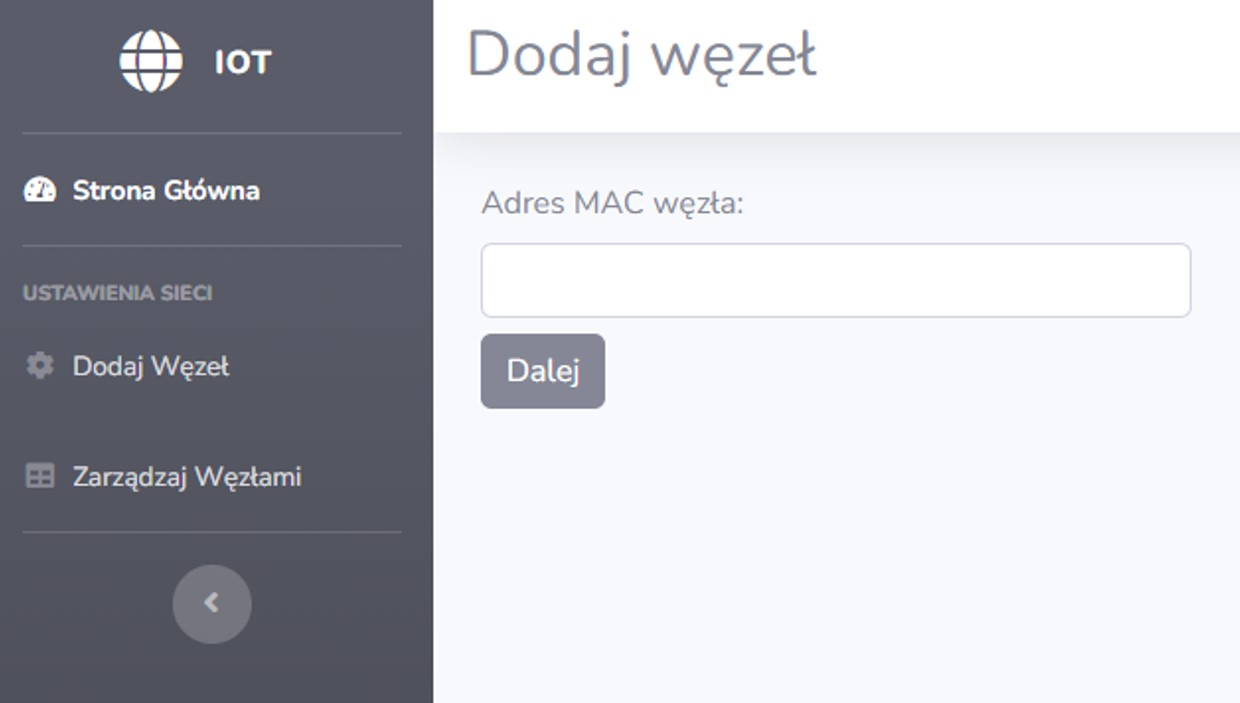
\includegraphics[scale=0.5]{test1}
\caption{Widok dodawania nowego węzła.}
\end{figure}
\par
Wprowadzenie adresu MAC modułu Bluetooth użytego do budowy węzła i kliknięcie „Dalej” sprawia, że aplikacja sprawdzi czy podany adres znajduje się w bazie danych a następnie zostanie wykonana procedura nawiązania łączności bezprzewodowej.  
\par
Po kilku chwilach, jeśli wszystko przebiegło pomyślnie aplikacja zwraca stosowny komunikat.
\begin{figure}[H]
\centering
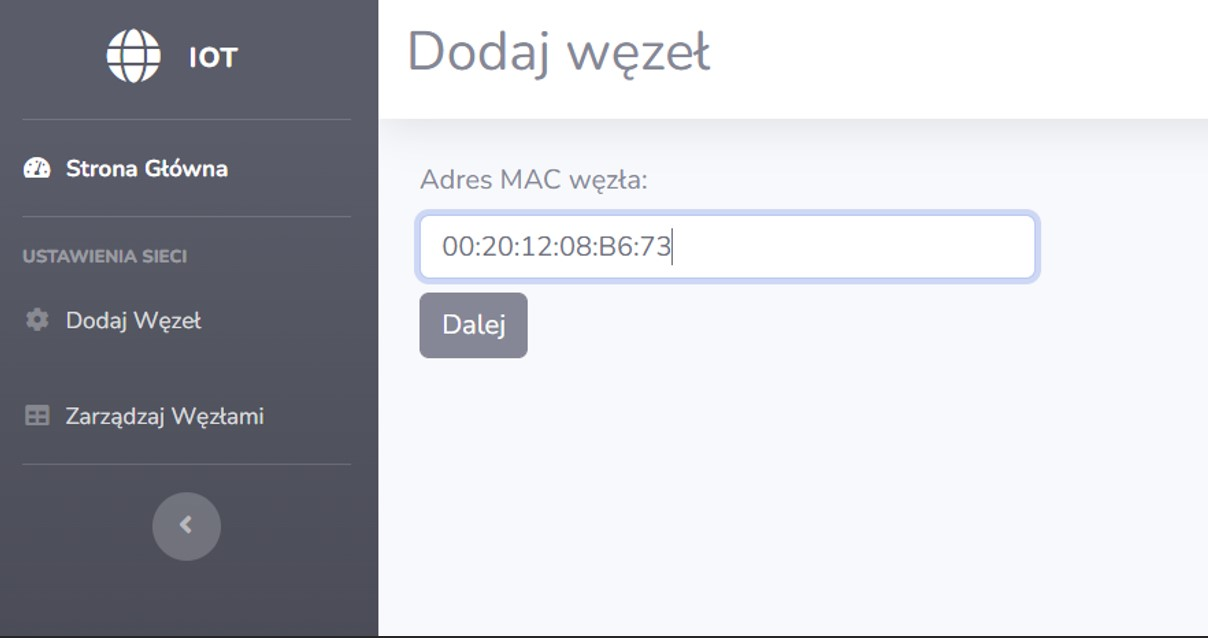
\includegraphics[scale=0.5]{test2}
\caption{Widok dodawania nowego węzła po wpisaniu adresu MAC.}
\end{figure}
\begin{figure}[H]
\centering
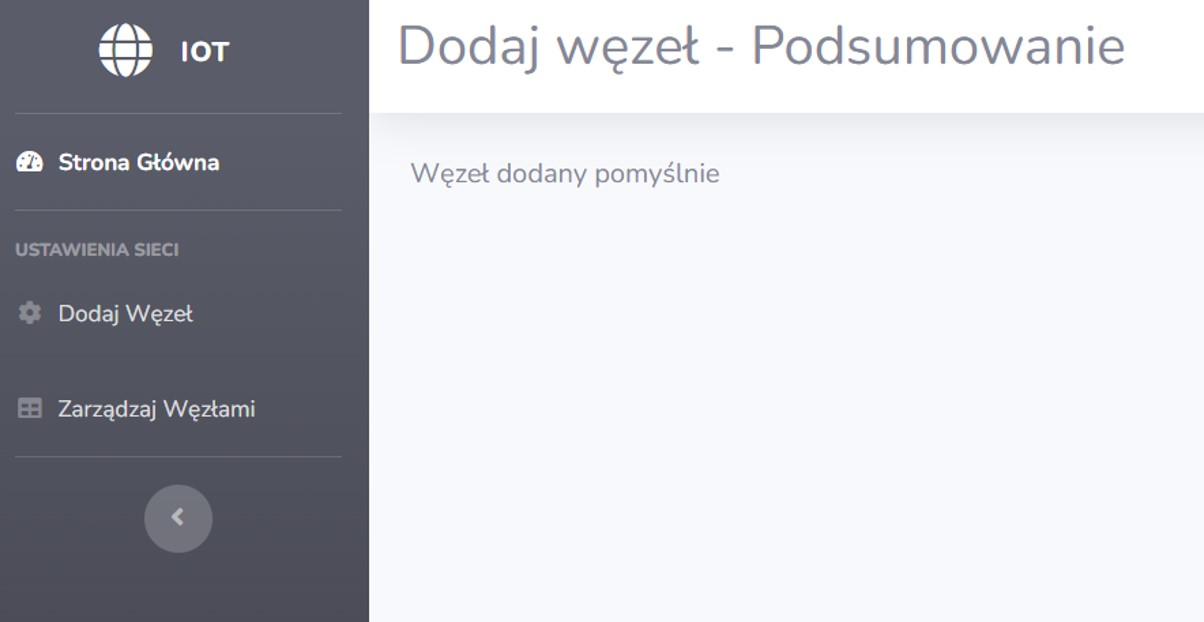
\includegraphics[scale=0.5]{test3}
\caption{Komunikat informujący o pomyślnym dodaniu węzła.}
\end{figure}
\par
Od tej pory dodany węzeł jest powiązany ze stacją i można uzyskać do niego dostęp poprzez zakładkę „Zarządzaj węzłami”
\begin{figure}[H]
\centering
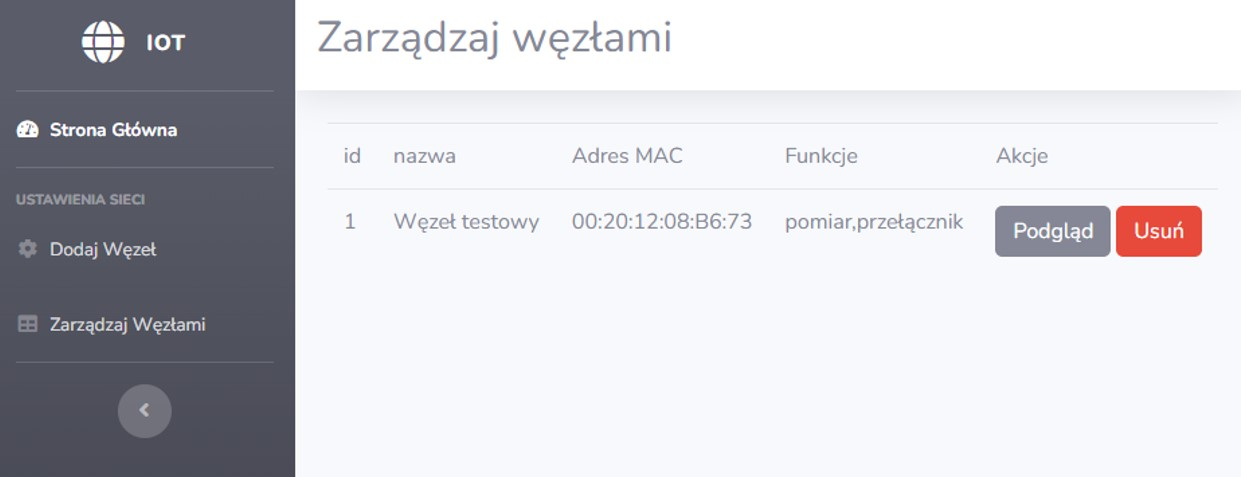
\includegraphics[scale=0.5]{test4}
\caption{Widok zarządzania węzłami}
\end{figure}
\par
Na rysunku 6.6 znajduje się tabela ze wszystkimi węzłami powiązanymi ze stacją. Znajduje się w niej id węzła, czyli unikatowy identyfikator przydzielony przez stacje oraz informacje pochodzące z bazy danych, czyli nazwa węzła i funkcje jakie pełni. W kolumnie „Akcje” znajduje się przycisk „Usuń” służący do usuwania węzła z tabeli oraz przycisk „Podgląd” który prowadzi do widoku służącego do komunikacji z węzłem. 
\begin{figure}[H]
\centering
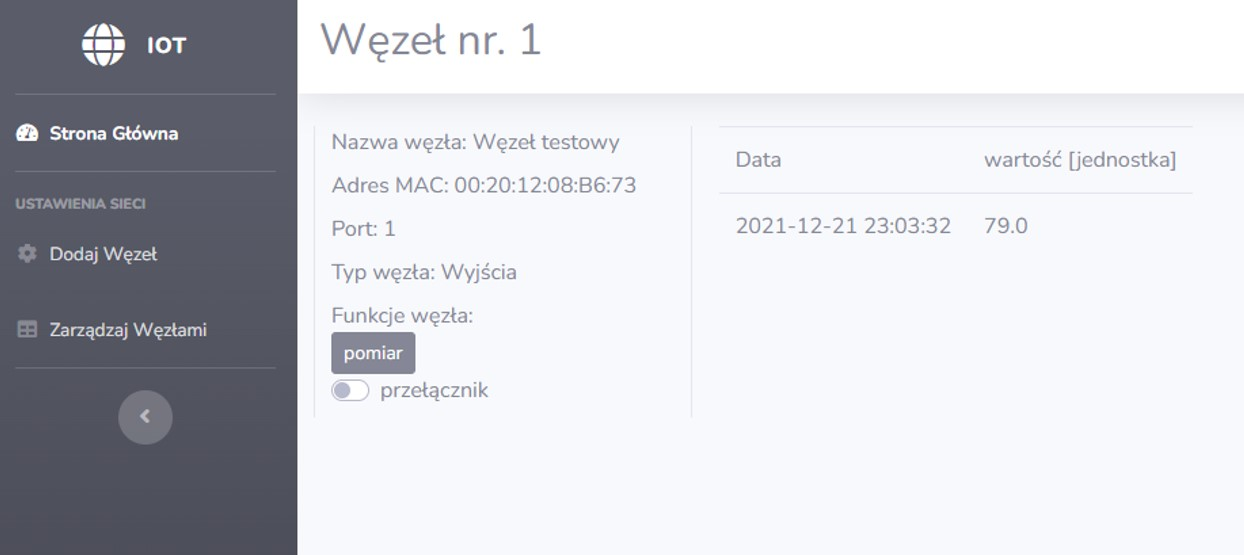
\includegraphics[scale=0.5]{test5}
\caption{Widok szczegółów dotyczących danego węzła}
\end{figure}
\par
Na rysunku 6.7 przedstawiono widok po wciśnięciu przycisku podgląd. Znajdują się w nim podstawowe informacje o węźle oraz elementy interfejsu służące do wydawania poleceń. Wywołanie metody, która odczyta wartość z bufora portu szeregowego i zapisze ją do bazy danych jest możliwe poprzez aktywowanie przycisku „pomiar”. Podobnie działa pole wyboru „przełącznik”. Po kliknięciu go przez użytkownika wysyłane jest żądanie do stacji usługowej, aby wydała ona polecenie węzłowi zgaszenia bądź zapalenia diody LED.

%---7----
\chapter{Podsumowanie}

W ramach projektu niniejszej pracy udało się osiągnąć cel projektu i spełnić wszystkie jego założenia. Realizacja projektu obejmowała następujące zagadnienia:
\begin{itemize}
\item	Konstrukcja dedykowanej stacji usługowej Internetu Rzeczy – skonfigurowano komputer jednopłytkowy poprzez zainstalowanie odpowiedniego oprogramowania tak aby przystosować urządzenie do pełnienia funkcji serwera www. Stworzono dedykowane oprogramowanie w tym:
\begin{itemize}
\item	 Skrypt w języku Python odpowiedzialny za procedurę nawiązywania łączności bezprzewodowej z wykorzystaniem standardu Bluetooth.
\item	Aplikacja Internetowa języka Python wraz z biblioteką Flask służąca do obsługi żądań protokołu HTTP pochodzących z przeglądarki.
\item	Warstwa wizualna aplikacji internetowej wyświetlana w przeglądarce opracowana przy pomocy takich technologii jak HTML i CSS oraz JavaScript.  
\item	Relacyjna baza danych oparta na standardzie SQL.
\end{itemize}
\item	Przeprowadzenie weryfikacji eksperymentalnej – wykazano negatywny wpływ zakłóceń takich jak obce sygnały w paśmie 2,4GHz na niezawodność komunikacji przy użyciu standardu Bluetooth. Zmierzono największą odległość, która gwarantuje bezbłędną transmisję w środowisku testowym którym był blok mieszkalny i wynosi ona 10 metrów. Pomiary powtórzono dla domu jednorodzinnego, czyli środowisku o znacząco mniejszej liczbie zbędnych sygnałów co poskutkowało zwiększeniem maksymalnego zasięgu o 20\%.
Ponad to dokonano testów manualnych wersji demonstracyjnej stacji usługowej. Udało się w pomyślnie ustanowić połączenie węzła ze stacją przy użyciu graficznego interfejsu użytkownika w postaci aplikacji Internetu. Urządzenie działa i posiada wszystkie założone funkcjonalności.
\end{itemize}

%----KONIEC------------------------

\begin{thebibliography}{99}
\bibitem[1]{} Dave Evans, "The Internet of Things: How the Next Evolution of the Internet Is Changing Everything", CISCO White Paper, kwiecień 2011, s. 3.
\bibitem[2]{} Smart Energy Efficient Home Automation System Using IoT, IEEE, 29 July 2019, DOI: 10.1109/IoT-SIU.2019.8777607
\bibitem[3]{} CRAIoT: Concept, Review and Application(s) of IoT, IEEE, 29 July 2019, DOI: 10.1109/IoT-SIU.2019.8777467
\bibitem[4]{} Sudhir K. Routray, Sharath Anand, NARROWBAND IOT FOR HEALTHCARE, IEEE, 19 October 2017, DOI: 10.1109/ICICES.2017.8070747
\bibitem[5]{} S. Rajendran, T. Hari Prasath, S. Revathi, K. Rajesh, Basic Food Safety Monitoring And Enhancement in Coffee Industry Using IOT, IEEE, 20 April 2021, DOI: 10.1109/ICACITE51222.2021.9404609
\bibitem[6]{} Mike O. Ojo, Stefano Giordano, Gregorio Procissi, Ilias N. Seitanidis, A Review of Low-End, Middle-End, and High-End Iot Devices, December 18, IEEE, 09 November 2018, DOI: 10.1109/ACCESS.2018.2879615
\bibitem[7]{} Yaxing Yao, Justin Reed Basdeo, Smirity Kaushik, YangWang, Defending My Castle: A Co-Design Study of Privacy Mechanisms for Smart Homes, IEEE, May 4–9, 2019, DOI: 10.1145/3290605.3300428
\bibitem[8]{} Hittu G., Mayank D., Securing IoT Devices and Securely Connecting the Dots Using REST API and Middleware, IEEE, 18-19 April 2019, DOI: 10.1109/IoT-SIU.2019.8777334
\bibitem[9]{} URL: https://www.statista.com/statistics/976313/global-iot-market-size/
\bibitem[10]{} bluetooth.org, Bluetooth Core Specification v.5.2, s.196, 2019-12-31
\bibitem[11]{} Rozporządzenie Ministra Administracji i Cyfryzacji z dnia 12 grudnia 2014 r. w sprawie urządzeń radiowych nadawczych lub nadawczo-odbiorczych, które mogą być używane bez pozwolenia radiowego. URL: http://isap.sejm.gov.pl/isap.nsf/DocDetails.xsp?id=WDU20170000096
\bibitem[12]{} 802.15 WPAN Task Group 6 Body Area Networks, IEEE, 13 January 2022 URL: https://www.ieee802.org/15/pub/TG6.html
\bibitem[13]{} Poslad Stefan, Ubiquitous Computing Smart Devices, Smart Environments and Smart Interaction, s. 15, 2009
\bibitem[14]{} Gratton, Dean A, The Handbook of Personal Area Networking Technologies and Protocols, Cambridge University Press. Strony 15–18, 2013 
\bibitem[15]{} Gary A. Donahue, Network Warrior, O'Reilly. s. 5, June 2007
\bibitem[16]{} Groth, David and Skandler, Toby, Network+ Study Guide, Fourth Edition, s. 121 June 2007
\bibitem[17]{} Dyrektywa Parlamentu Europejskiego i Rady 2014/53/UE z dnia 16 kwietnia 2014 r. w sprawie harmonizacji ustawodawstw państw członkowskich dotyczących udostępniania na rynku urządzeń radiowych i uchylająca dyrektywę
\bibitem[18]{} Nyein Aye Maung Maung , Win Zaw, Comparative Study of RSS-based Indoor Positioning Techniques on Two Different Wi-Fi Frequency Bands, IEEE, 24-27 June 2020, DOI: 10.1109/ECTI-CON49241.2020.9158211
\bibitem[19]{} Dilip Geevarghese, BLE vs Wi-Fi: Which is Better for IoT Product Development?, February 01, 2018, URL:  https://www.cabotsolutions.com/ble-vs-wi-fi-which-is-better-for-iot-product-development
\bibitem[20]{} Bradley Mitchell, How Fast Is a Wi-Fi Network?, June 16 2021
\bibitem[21]{} bluetooth.com, Understanding Bluetooth Range, \par URL: https://www.bluetooth.com/learn-about-bluetooth/key-attributes/range/
\bibitem[22]{} HC-05 Bluetooth Module User’s Manual V1.0 URL: https://www.gme.cz/data/attachments/dsh.772-148.1.pdf
\bibitem[23]{} raspberrypi.org, Raspberry Pi 4 Computer Model B – product brief
\end{thebibliography}

\listoffigures

\listoftables

\listofalgorithms
%----Bibliografia------------------

\end{document}

